\documentclass[unicode,11pt,a4paper,oneside,numbers=endperiod,openany]{scrartcl}
\usepackage{ifthen}
\usepackage[utf8]{inputenc}
\usepackage{graphics}
\usepackage{graphicx}
\usepackage{hyperref}

\pagestyle{plain}
\voffset -5mm
\oddsidemargin  0mm
\evensidemargin -11mm
\marginparwidth 2cm
\marginparsep 0pt
\topmargin 0mm
\headheight 0pt
\headsep 0pt
\topskip 0pt        
\textheight 255mm
\textwidth 165mm

\newcommand{\duedate} {}
\newcommand{\setduedate}[1]{%
\renewcommand\duedate {See iCorsi for due date}}
\newcommand\isassignment {false}
\newcommand{\setassignment}{\renewcommand\isassignment {true}}
\newcommand{\ifassignment}[1]{\ifthenelse{\boolean{\isassignment}}{#1}{}}
\newcommand{\ifnotassignment}[1]{\ifthenelse{\boolean{\isassignment}}{}{#1}}

\newcommand{\assignmentpolicy}{
\begin{table}[h]
\begin{center}
\scalebox{0.8} {%
\begin{tabular}{|p{0.02cm}p{16cm}|}
\hline
&\\
\multicolumn{2}{|c|}{\Large\textbf{HPC Lab ---  Submission Instructions}}\\
\multicolumn{2}{|c|}{\large\textbf{(Please, notice that following instructions are mandatory: }}\\
\multicolumn{2}{|c|}{\large\textbf{submissions that don't comply with, won't be considered)}}\\
&\\
\textbullet & Assignments must be submitted to \href{https://www.icorsi.ch}{iCorsi} (i.e. in electronic format).\\
\textbullet & Provide both executable package and sources (e.g. C/C++ files, Matlab). 
If you are using libraries, please add them in the file. Sources must be organized in directories called:\\
\multicolumn{2}{|c|}{\textit{Project\_number\_lastname\_firstname}}\\
& and  the  file must be called:\\
\multicolumn{2}{|c|}{\textit{project\_number\_lastname\_firstname.zip}}\\
\multicolumn{2}{|c|}{\textit{project\_number\_lastname\_firstname.pdf}}\\
\textbullet &  The TAs will grade your project by reviewing your project write-up, and looking at the implementation 
                 you attempted, and benchmarking your code's performance.\\

\textbullet & You are allowed to discuss all questions with anyone you like; however: (i) your submission must list anyone you discussed problems with and (ii) you must write up your submission independently.\\
\hline
\end{tabular}
}
\end{center}
\end{table}
}
\newcommand{\punkte}[1]{\hspace{1ex}\emph{\mdseries\hfill(#1~\ifcase#1{Points}\or{Points}\else{Points}\fi)}}


\newcommand\serieheader[6]{
\thispagestyle{empty}%
\begin{flushleft}

\includegraphics[width=0.4\textwidth]{media/usi_inf.png}
\end{flushleft}
  \noindent%
  {\large\ignorespaces{\textbf{#1}}\hspace{\fill}\ignorespaces{ \textbf{#2}}}\\ \\%
  {\large\ignorespaces #3 \hspace{\fill}\ignorespaces #4}\\
  \noindent%
  \bigskip
  \hrule\par\bigskip\noindent%
  \bigskip {\ignorespaces {\Large{\textbf{#5}}}
  \hspace{\fill}\ignorespaces \large \ifthenelse{\boolean{\isassignment}}{\duedate}{#6}}
  \hrule\par\bigskip\noindent%  \linebreak
 }

\makeatletter
\def\enumerateMod{\ifnum \@enumdepth >3 \@toodeep\else
      \advance\@enumdepth \@ne
      \edef\@enumctr{enum\romannumeral\the\@enumdepth}\list
      {\csname label\@enumctr\endcsname}{\usecounter
        {\@enumctr}%%%? the following differs from "enumerate"
	\topsep0pt%
	\partopsep0pt%
	\itemsep0pt%
	\def\makelabel##1{\hss\llap{##1}}}\fi}
\let\endenumerateMod =\endlist
\makeatother




\usepackage{textcomp}





\usepackage{ntheorem}
\usepackage{subcaption}
\usepackage{booktabs}
\usepackage{multirow}
\usepackage{tabularx}
\usepackage{listings}
\usepackage{amsmath}
\usepackage{graphicx}
\usepackage{float}
\usepackage{epstopdf} %converting to PDF
\usepackage[dvipsnames]{xcolor}
\usepackage[
	backend=biber,
]{biblatex}
\addbibresource{bib/sources.bib}
\theoremstyle{plain}
\theorembodyfont{\upshape} % or "\itshape", or whatever
\newtheorem{question}{Question}

\definecolor{codegreen}{rgb}{0,0.6,0}
\definecolor{codegray}{rgb}{0.5,0.5,0.5}
\definecolor{codepurple}{rgb}{0.58,0,0.82}
\definecolor{codeblue}{rgb}{0.251, 0.471, 0.753}
\definecolor{backcolour}{rgb}{0.961, 0.961, 0.961}

\lstdefinestyle{mystyle}{%
    backgroundcolor=\color{backcolour},   
    commentstyle=\color{Fuchsia}\textit,
    keywordstyle=\color{NavyBlue},
    numberstyle=\tiny\color{codegray},
    stringstyle=\color{Green},
    basicstyle=\ttfamily\footnotesize,
    breakatwhitespace=false,         
    breaklines=true,                 
    captionpos=b,                    
    keepspaces=true,                 
    numbers=left,                    
    numbersep=5pt,                  
    showspaces=false,                
    showstringspaces=false,
    showtabs=false,                  
    tabsize=2,
}


\lstset{style=mystyle}

\begin{document}

\setassignment

\serieheader{High-Performance Computing Lab}{Institute of Computing}{Student: Dennys Mike Huber}{Discussed with: Alberto Finardi \& Leon Ackermann}{Solution for Project 6}{}
\newline
In this project, we will investigate the graph partitioning problem within the context of domain decomposition for high-performance computing (HPC) applications.
\section{Construct adjacency matrices from connectivity data [10 points]}
For this exercise the goal was to read the csv file of each graph and create a sparse adjacency matrix which must symmetric and sparse.
To ensure the first property  we applied the code seen in Listing \ref{lst:sym}, where we check if the matrix is symmetric and if not do the necessary adjustment.
To ensure the second property we use the \texttt{sparse} function to create a sparse matrix.
\begin{lstlisting}[language=Matlab, caption=Ensure symmetric property, label=lst:sym]
W = sparse(from,to, 1, nodes, nodes);
if ~issymmetric(W)
	W = (W+W')/2;
	disp('The adjacency matrix has been symmetrized.');
end
\end{lstlisting}

\begin{figure}[H]
	\centering
	\begin{subfigure}{0.5\textwidth}
		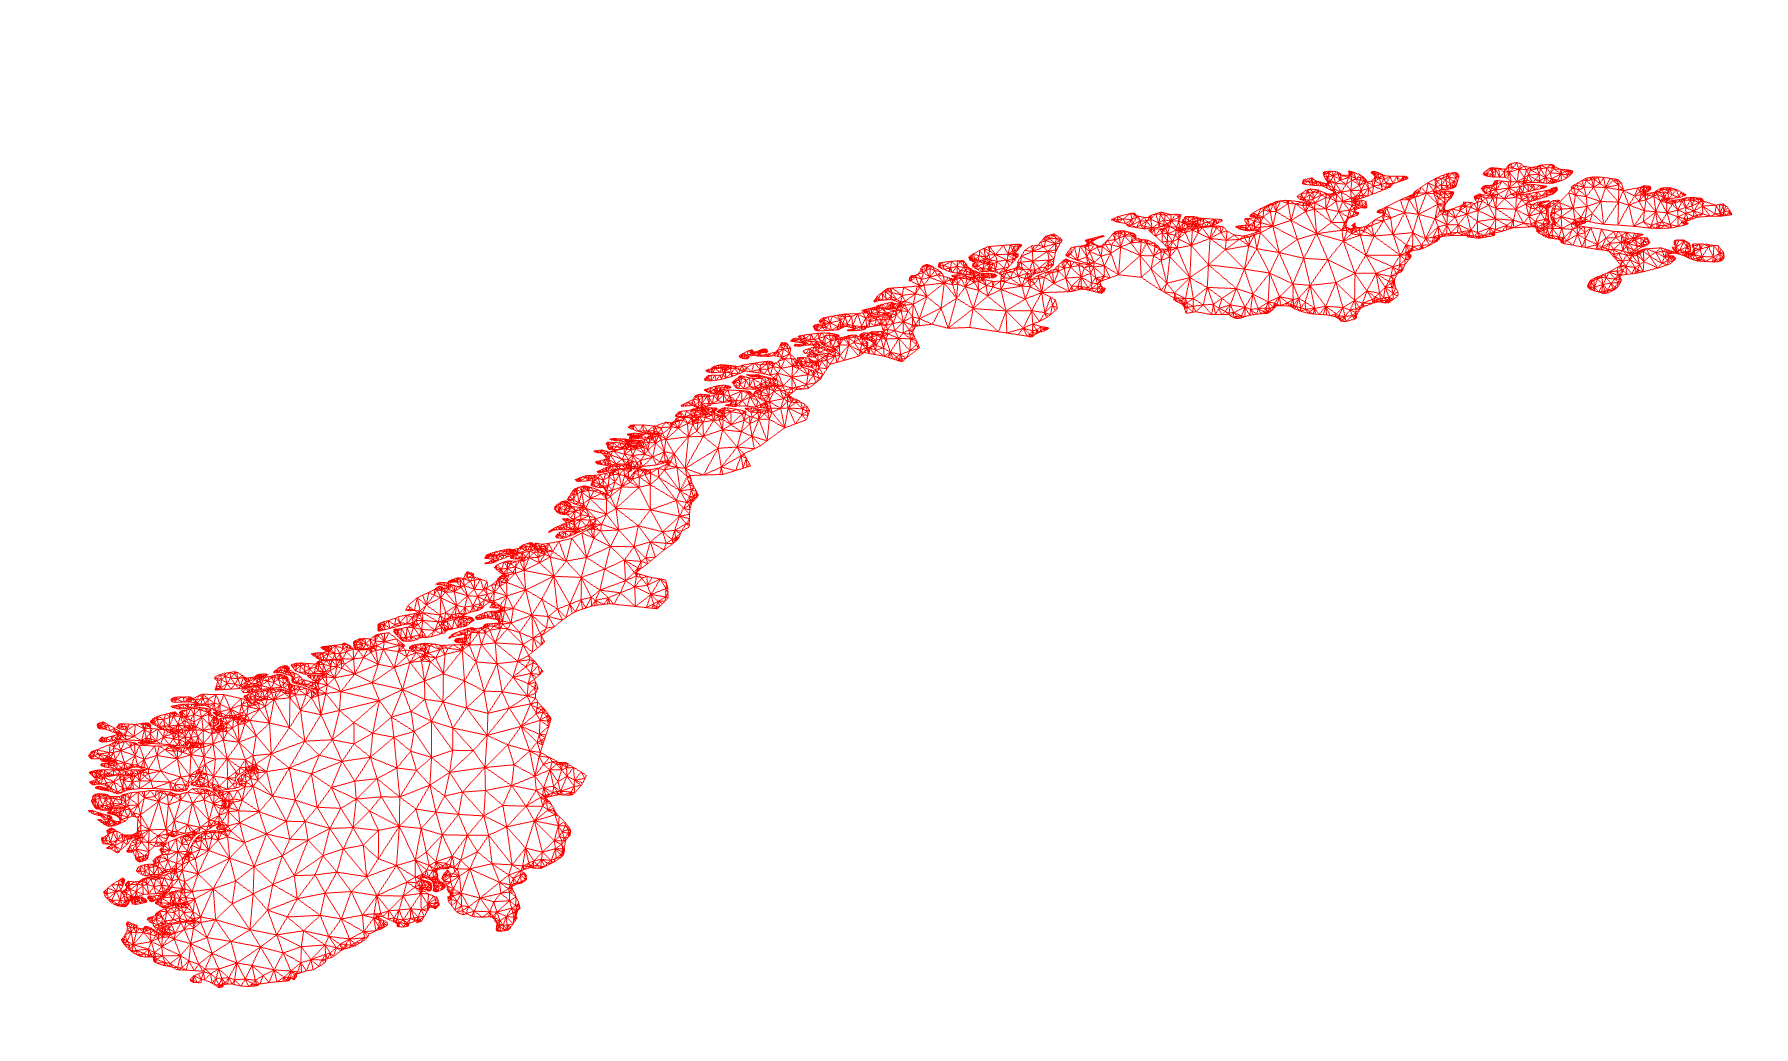
\includegraphics[width=\textwidth]{./media/norway.png}
		\caption{Norway}
		\label{fig:no}
	\end{subfigure}%
    ~
	\begin{subfigure}{0.5\textwidth}
		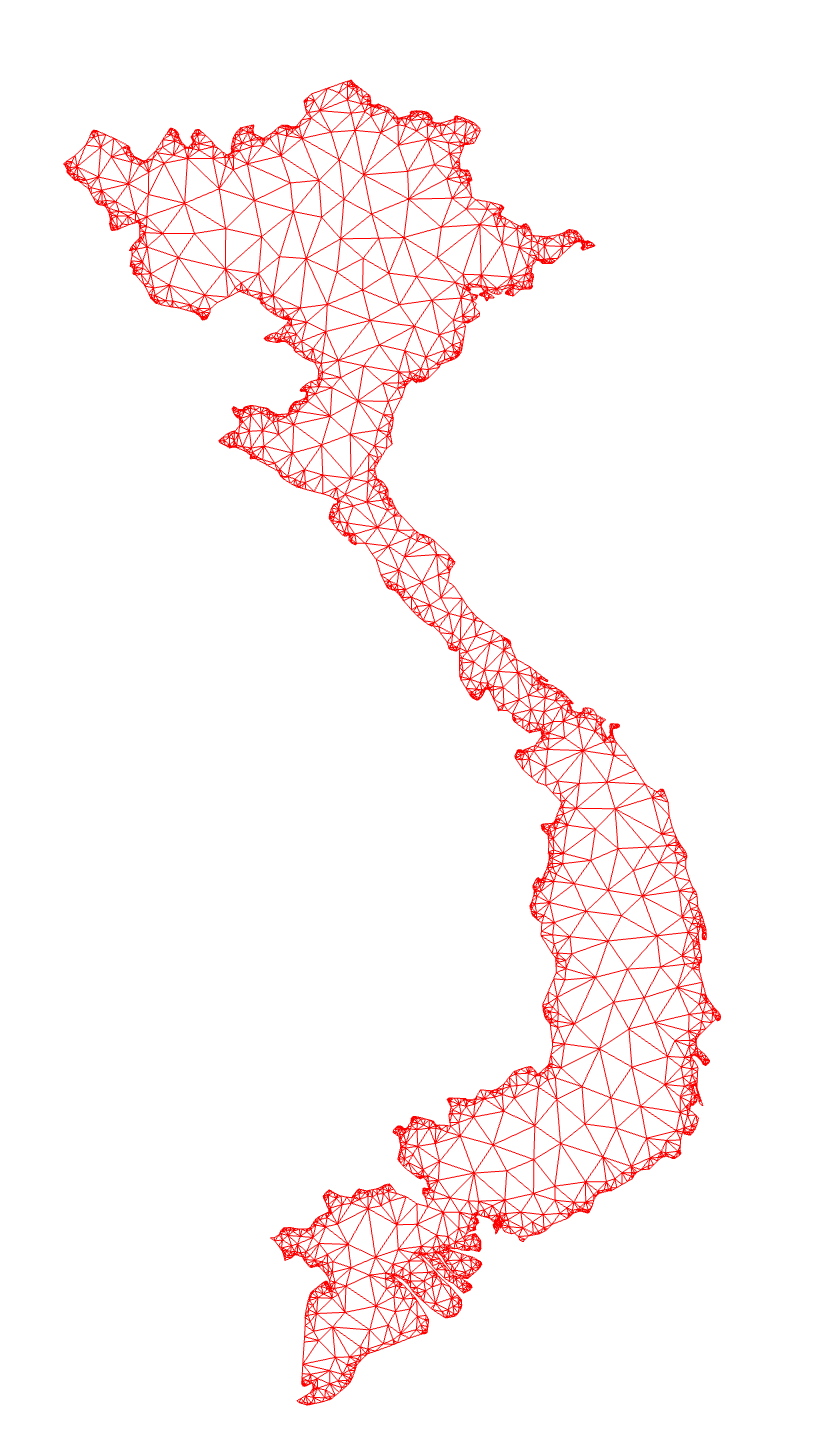
\includegraphics[width=0.5\textwidth]{./media/vietnam.png}
		\caption{Vietnam}
		\label{fig:viet}
	\end{subfigure}
	\caption{Country graphs}
	\label{fig:countries}
\end{figure}
After creating the adjacency matrix we save it and the coordinates matrix in folder \texttt{./Datasets/Countries\_Mat}. As the final step we load the matrices for Norway and Vietnam and visualize it with the provided \texttt{gplotg} function. The resulting graphs can be seen in Figure \ref{fig:countries}.


\section{Optimize Square Matrix-Matrix Multiplication  \punkte{50}}
\subsection{Implementation}
As given in the exercise, the optimal block size is
\begin{equation}
	s = \sqrt{\frac{M}{3}}
\end{equation}
where $M$ is the size of the fast memory. In our case this is the size of the L1 cache, which is 32KB as seen in table \ref{tab:cache}. In our dgemm-blocked implementation we use the double type, which has size 64 bit or 8 byte. Therefore we can convert our L1 cache size into bytes and divide it by the size of the double type in order to get $M$.
\begin{equation}
	M = \frac{32000}{8} = 4000 \ \text{doubles}
\end{equation}
After finding $M$, we can now calculate $s$:
\begin{equation}
	s = \sqrt{\frac{4000}{3}} = 36.5148 \approx 36 \ \text{blocks}
\end{equation}
We can now insert this result into the blocked dgemm code given in Listing \ref{lst:dgemm}.
Shifting our attention to the actual implementation of Blocked dgemm.
The goal is to improve cache utilization by optimizing the memory access pattern and reduce cache misses.\newline
The two outer loops split the matrix up into smaller blocks of the previously calculated block sizes $s$.
The next two inner loops go through the individual entry of each block and make sure if the final block cannot be completely filled due to the matrix dimension, that there's not an out-of-bounds error. The innermost loop iterates over the shared dimension.
Finally the computation is then performed according to the column-major format. 
Notice that an additional variable sum is introduced, which reduces the times we have to write to the C matrix.
\begin{lstlisting}[language=C++, caption=Dgemm blocked, label=lst:dgemm]
 const char *dgemm_desc = "Blocked dgemm.";

// Optimize for single core
#define BLOCK_SIZE 36

/* This routine performs a dgemm operation
 *
 *  C := C + A * B
 *
 * where A, B, and C are lda-by-lda matrices stored in column-major format.
 * On exit, A and B maintain their input values.
 */
void square_dgemm(int n, double *A, double *B, double *C) {
  double sum;
  for (int bi = 0; bi < n; bi += BLOCK_SIZE) {
    for (int bj = 0; bj < n; bj += BLOCK_SIZE) {
      for (int i = bi; i < bi + BLOCK_SIZE && i < n; i++) {
        for (int j = bj; j < bj + BLOCK_SIZE && j < n; j++) {
          sum = C[i + j * n];
          for (int k = 0; k < n; k++) {
            sum += A[i + k * n] * B[k + j * n];
          }
          C[i + j * n] = sum;
        }
      }
    }
  }
}
 \end{lstlisting}
This initial dgemm block implementation shows a significant improvement compared to the naive dgemm implementation as depicted in Figure \ref{fig:dgemm-0}
\begin{figure}[H]
	\centering
	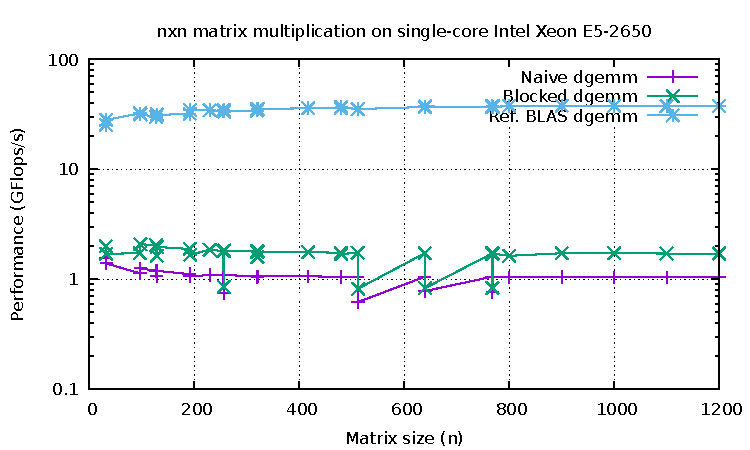
\includegraphics[width=\textwidth]{../media/timing-36.pdf}
	\caption{Timing of initial block matrix implementation}
	\label{fig:dgemm-0}
\end{figure}

\subsection{Unrolling Loops and Pragma statements}
As an attempt of improving the performance further, the innermost loop was replaced by the unrolled loop seen in Listing \ref{lst:unrolled}.
This loop is unrolled by a factor of 4, because this is equivalent to the number of doubles the FPU can process concurrently with a single SIMD instruction.
\begin{lstlisting}[language=C++, caption=Unrolled loop, label=lst:unrolled]
int k;
for (k = 0; k <= n - 4; k += 4) {
	sum += A[i + k * n] * B[k + j * n];
	sum += A[i + (k + 1) * n] * B[(k + 1) + j * n];
	sum += A[i + (k + 2) * n] * B[(k + 2) + j * n];
	sum += A[i + (k + 3) * n] * B[(k + 3) + j * n];
}
// For the final block if the number of elements is not divisible by 4
for (; k < n; k++) {
	sum += A[i + k * n] * B[k + j * n];
}
\end{lstlisting}
As a second approach the \texttt{\#pragma gcc ivdep} \cite{noauthor_loop-specific_nodate} directive was introduced in order to force the compiler to unconditionally vectorize the innermost loop.
Both approach did not show any improvement in performance compared to the initial block matrix implementation in Figure \ref{fig:dgemm-0}.
Hence these approaches were subsequently removed from my final blocked dgemm implementation, but the output file for this option can be found in the submission.
These approaches were most likely unsuccessful due to the compiler being able of doing these optimization on its own. This theory is reinforced by having a look at the provided compiler flags in the \texttt{Makefile} this includes flags such as \texttt{-funroll-loops} and \texttt{-march=native}.

\subsection{Compiler Flags}
By introducing further compiler flags, it is possible to increase the performance even more. Especially the addition of \texttt{-ffast-math} \cite{noauthor_floatingpointmath_nodate} resulted in an significant uptick in performance, see Figure \ref{fig:dgemm-fm}. It enables a set of flag that enables aggressive floating-point optimizations, but be aware \texttt{-ffast-math} is not always safe.
\begin{figure}[H]
	\centering
	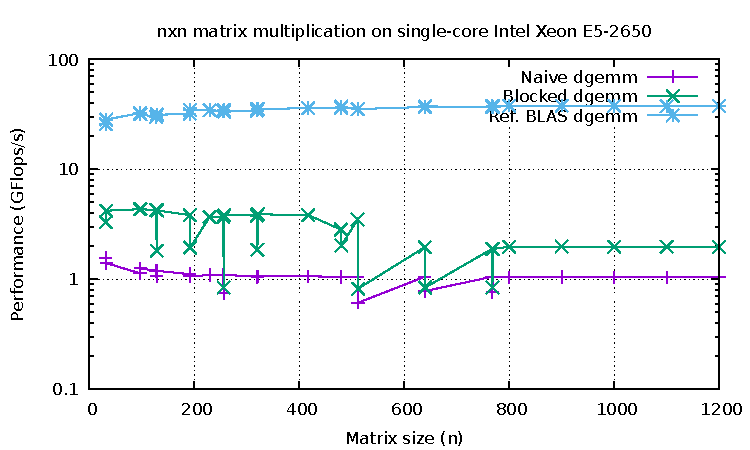
\includegraphics[width=\textwidth]{../media/timing-36-fast-math.pdf}
	\caption{Timing of dgemm using ffast-math}
	\label{fig:dgemm-fm}
\end{figure}



\section{Parallel histogram calculation using OpenMP}
In this exercise we will be analyzing the strong scaling of the parallel implementation of the histogram computation. The measured timings can be found in Table \ref{tab:hist-scaling}.
Because this is strong scaling analysis we kept the array size of the vector constant at $2 \cdot 10^9$ throughout the tests.\newline
The serial execution provides us with a baseline for comparison with the parallelized versions.
The single threaded execution shows a minor increase in performance, which is unexpected, due to the fact that there should be an overhead due to the thread management. This  indicates that the overhead was somehow less significant and it could be based on the workload of the cluster.
As we increase the number of threads, between 2 and 8 threads, we can observe a significant reduction in execution time, which indicates efficient scaling, when the workload is distributed over an increasing number of threads.\newline
When comparing the timing from 8 to 16 threads, the execution time still slightly decreases, but at much lower rate than before. This leads to the conclusion that the efficiency decreases and the thread management overhead and potential contention between threads for shared resources.\newline
From 32 onwards the timing increases, which means that the overhead outweighs the benefits gained from parallelizing the code. Another important factor that plays into the slower execution time is that the node only has 20 cores, resulting in more threads than cores, which means that certain threads potentially have to wait their turn until they can execute their chunk of code.
\begin{table}[H]
	\centering
	\begin{tabular}{|c|c|}
		\hline
		\textbf{Threads} & \textbf{Timing} \\ \hline
		Serial           & 0.839258s       \\ \hline
		1                & 0.830452s       \\ \hline
		2                & 0.418288s       \\ \hline
		4                & 0.213519s       \\ \hline
		8                & 0.110719s       \\ \hline
		16               & 0.112852s       \\ \hline
		32               & 0.120083s       \\ \hline
		64               & 0.127492s       \\ \hline
		128              & 0.129270s        \\ \hline
	\end{tabular}
	\caption{Execution time for strong scaling parallel histogram calculation}
	\label{tab:hist-scaling}
\end{table}


\newpage
\section{Comparing recursive bisection to direct k-way partitioning [10 points]}
In this exercise the goal is to compare and analyze the performance of recursive bisection and direct k-way partitioning by looking at the edge cut result. Both methods are using Metis and the goal is to partition the graphs into 16 (Table~\ref{tab:partitions_rec}) and 32 (Table~\ref{tab:partitions_k_way}) partitions. Comparing the two methods we can clearly see that that direct k-way partitioning consistently outperforms the recursive bisection by creating a smaller edge cut. This is the case because recursive bisection has no global information when doing partitioning decisions, k-way on the other hand overcomes this limitation by coarsening the graph first and the then refining the partitioning. Knowing this coarsening and refinement steps it was anticipated that k-way partitioning would outperform recursive bisection. Another observation that can be made is that the difference in edge cut between the methods increases when comparing 16 to 32 partitions. Indicating that k-way multiway partitioning also scales better in terms of number of partitions.
\begin{table}[H]
	\centering
	\begin{tabular}{lccccccc} % Note the number of columns matches the data
		\toprule
		Partitions & Luxemburg & USRoads & Greece & Switzerland & Vietnam & Norway & Russia \\
		\midrule
		16         & 191       & 585        & 318    & 685         & 270     & 271    & 572    \\
		32         & 317       & 983        & 500    & 1067        & 445     & 509    & 941    \\
		\bottomrule
	\end{tabular}
	\caption{Cut edges for recursive bisection.}
	\label{tab:partitions_rec}
\end{table}

\begin{table}[H]
	\centering
	\begin{tabular}{lccccccc} % Ensure this matches your data columns
		\toprule
		Partitions & Luxemburg & USRoads & Greece & Switzerland & Vietnam & Norway & Russia \\
		\midrule
		16         & 185       & 545        & 301    & 665         & 231     & 241    & 551    \\
		32         & 304       & 921        & 486    & 1013        & 418     & 436    & 931    \\
		\bottomrule
	\end{tabular}
	\caption{Cut edges for direct multiway partitioning in Metis 5.0.2.}
	\label{tab:partitions_k_way}
\end{table}
Figure~\ref{fig:metis} showcases how various examples of graphs are partitioned differently when using recursive or k-way partitioning.

\begin{figure}[H]
	\centering
	\begin{subfigure}{0.5\textwidth}
		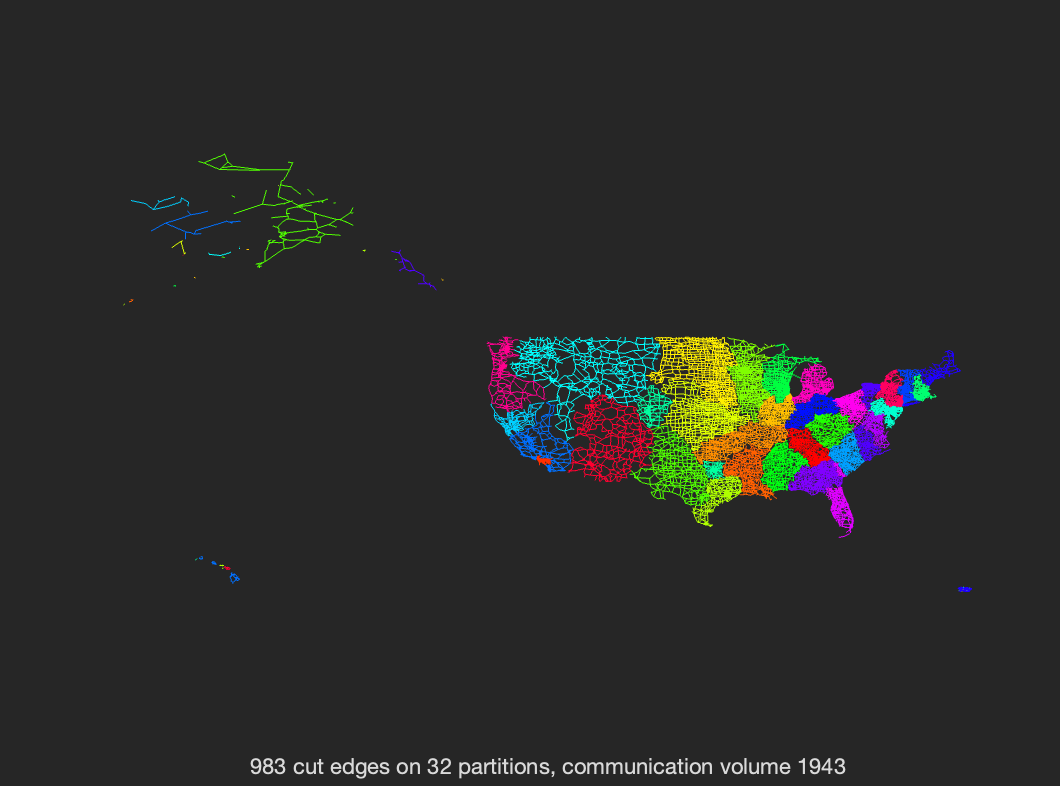
\includegraphics[width=\textwidth]{./media/usa_metis.png}
		\caption{USA with recursive bisection}
		\label{fig:usa_metis}
	\end{subfigure}%
	~
	\begin{subfigure}{0.5\textwidth}
		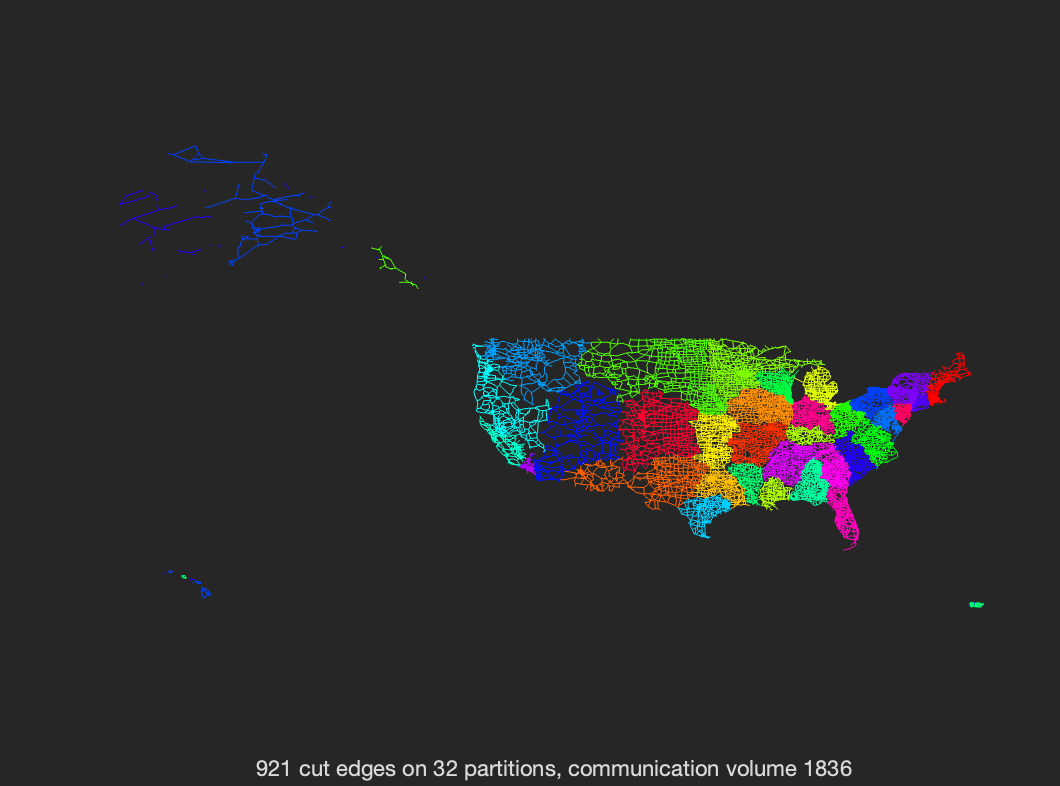
\includegraphics[width=\textwidth]{./media/usa_metis_k.png}
		\caption{USA with direct multiway partitioning}
		\label{fig:usa_metis_k}
	\end{subfigure}\\
	\begin{subfigure}{0.5\textwidth}
		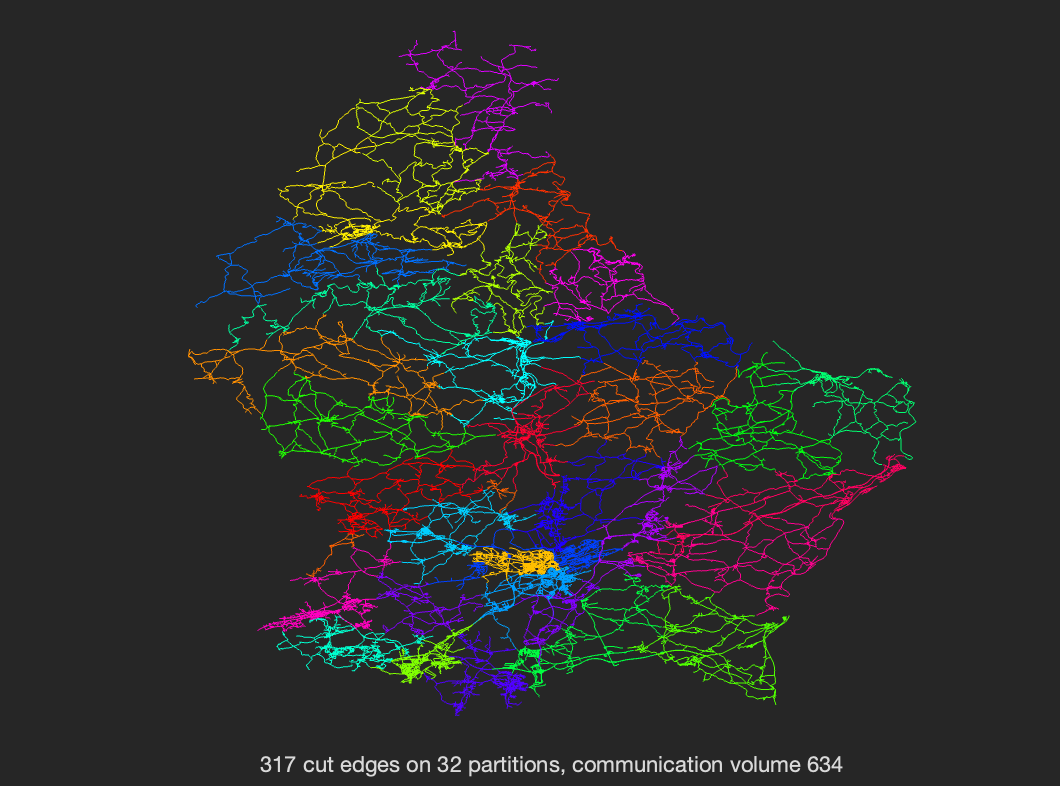
\includegraphics[width=\textwidth]{./media/lux_metis.png}
		\caption{Luxembourg with recursive bisection}
		\label{fig:lux_metis}
	\end{subfigure}%
	~
	\begin{subfigure}{0.5\textwidth}
		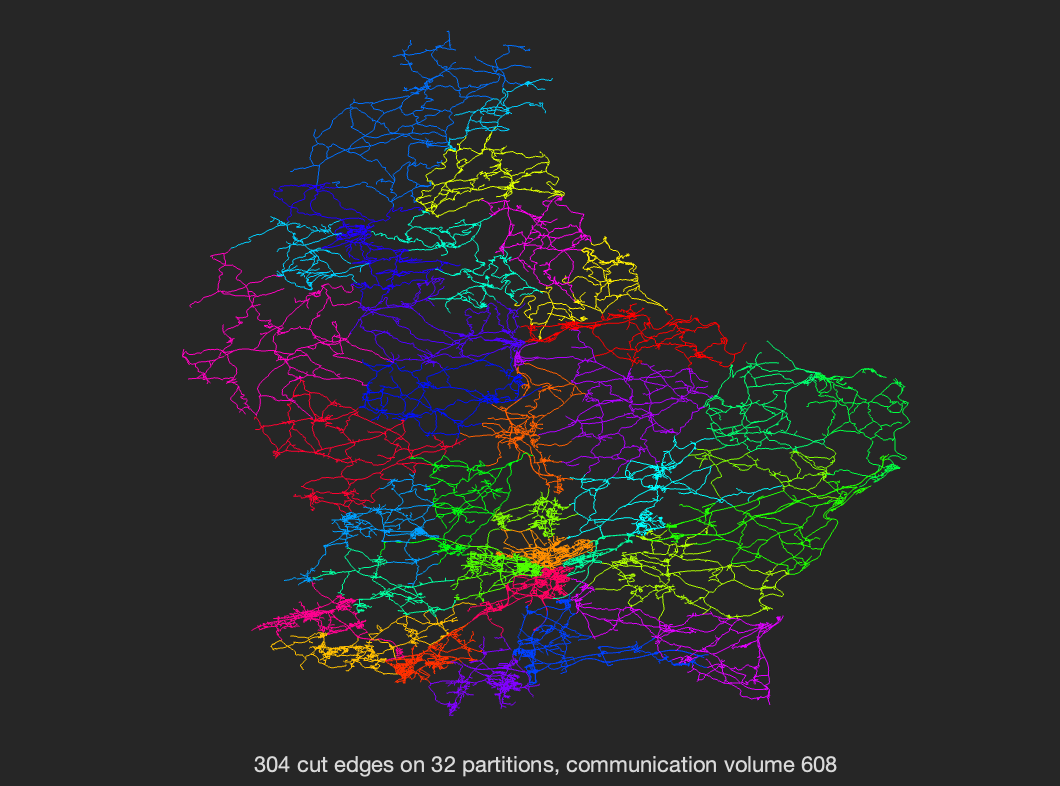
\includegraphics[width=\textwidth]{./media/lux_metis_k.png}
		\caption{Luxembourg with direct multiway partitioning}
		\label{fig:lux_metis_k}
	\end{subfigure}
	\begin{subfigure}{0.5\textwidth}
		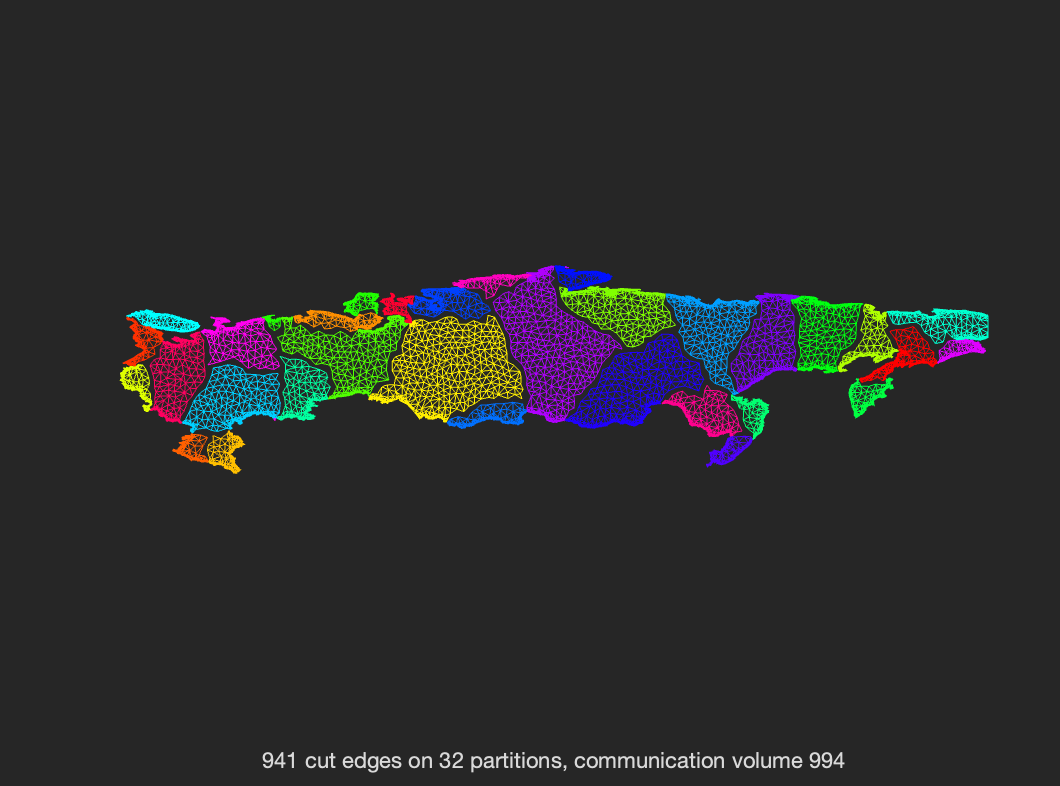
\includegraphics[width=\textwidth]{./media/ru_metis.png}
		\caption{Russia with recursive bisection}
		\label{fig:ru_metis}
	\end{subfigure}%
	~
	\begin{subfigure}{0.5\textwidth}
		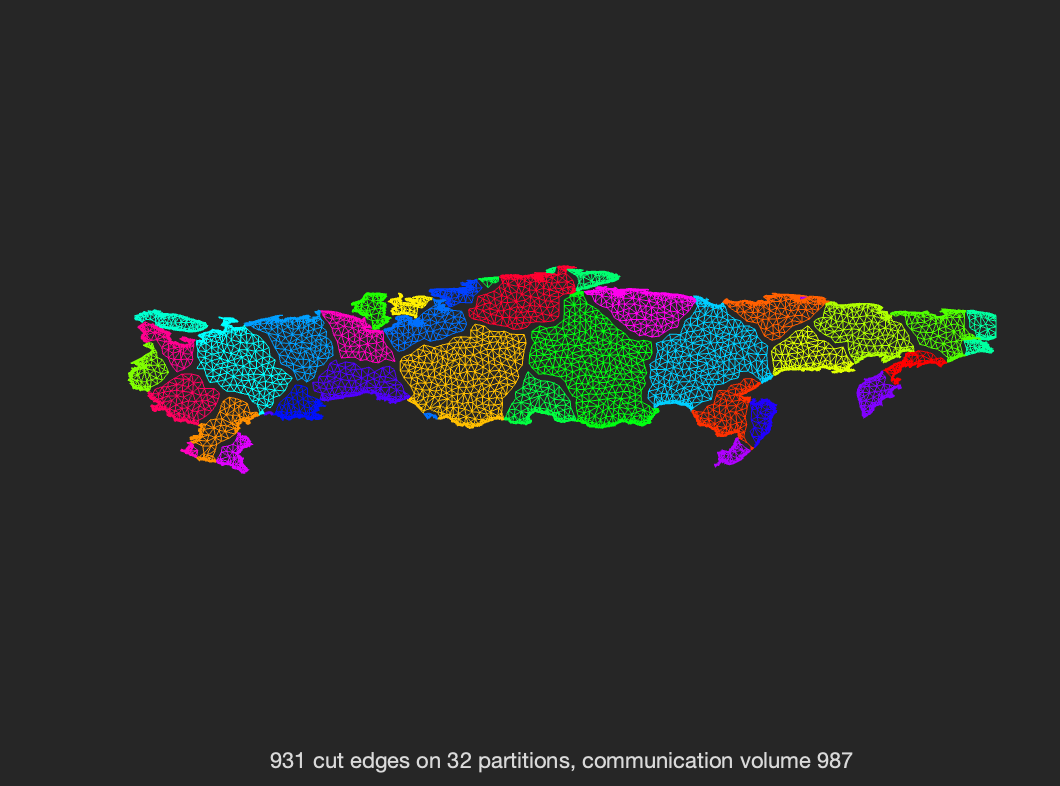
\includegraphics[width=\textwidth]{./media/ru_metis_k.png}
		\caption{Russia with direct multiway partitioning}
		\label{fig:ru_metis_k}
	\end{subfigure}

	\caption{Partitioning results for the graphs of USA, Luxemburg, and Russia
for 32 partitions}
	\label{fig:metis}
\end{figure}


\newpage
\section{Utilizing graph eigenvectors [25 points]}
The entries of the eigenvector associated with the first ($\lambda_1$) and second ($\lambda_2$) smallest of the Laplacian $L$ are plotted in Figure~\ref{fig:eig}. The behaviour of the $\lambda_1$'s eigenvector $v_1$ is expected to have only 1's as its elements due to the property of the $L$. In our case the entries are not 1 but the normalized vector which is  $\frac{v_1}{\sqrt{n}}$, where $n$ is the length of the eigenvector \cite{noauthor_smallest_nodate}. The Fiedler vector $v_2$ of the second smallest eigen value reflects the structure of the graph. Vertices are strongly connected will have similar eigenvector values, while vertices will show more distinct values, when they are further apart. When looking at plot for $v_2$ in the Subfigure \ref{sfig:eig2} you can see that the vector shows a smooth transition from positive to negative indicating that they are transitioning from one partition to another. Subfigure \ref{sfig:eig1} then shows this grouping using coloring of the vertices.
\begin{figure}[H]
	\centering
	\begin{subfigure}{0.5\textwidth}
		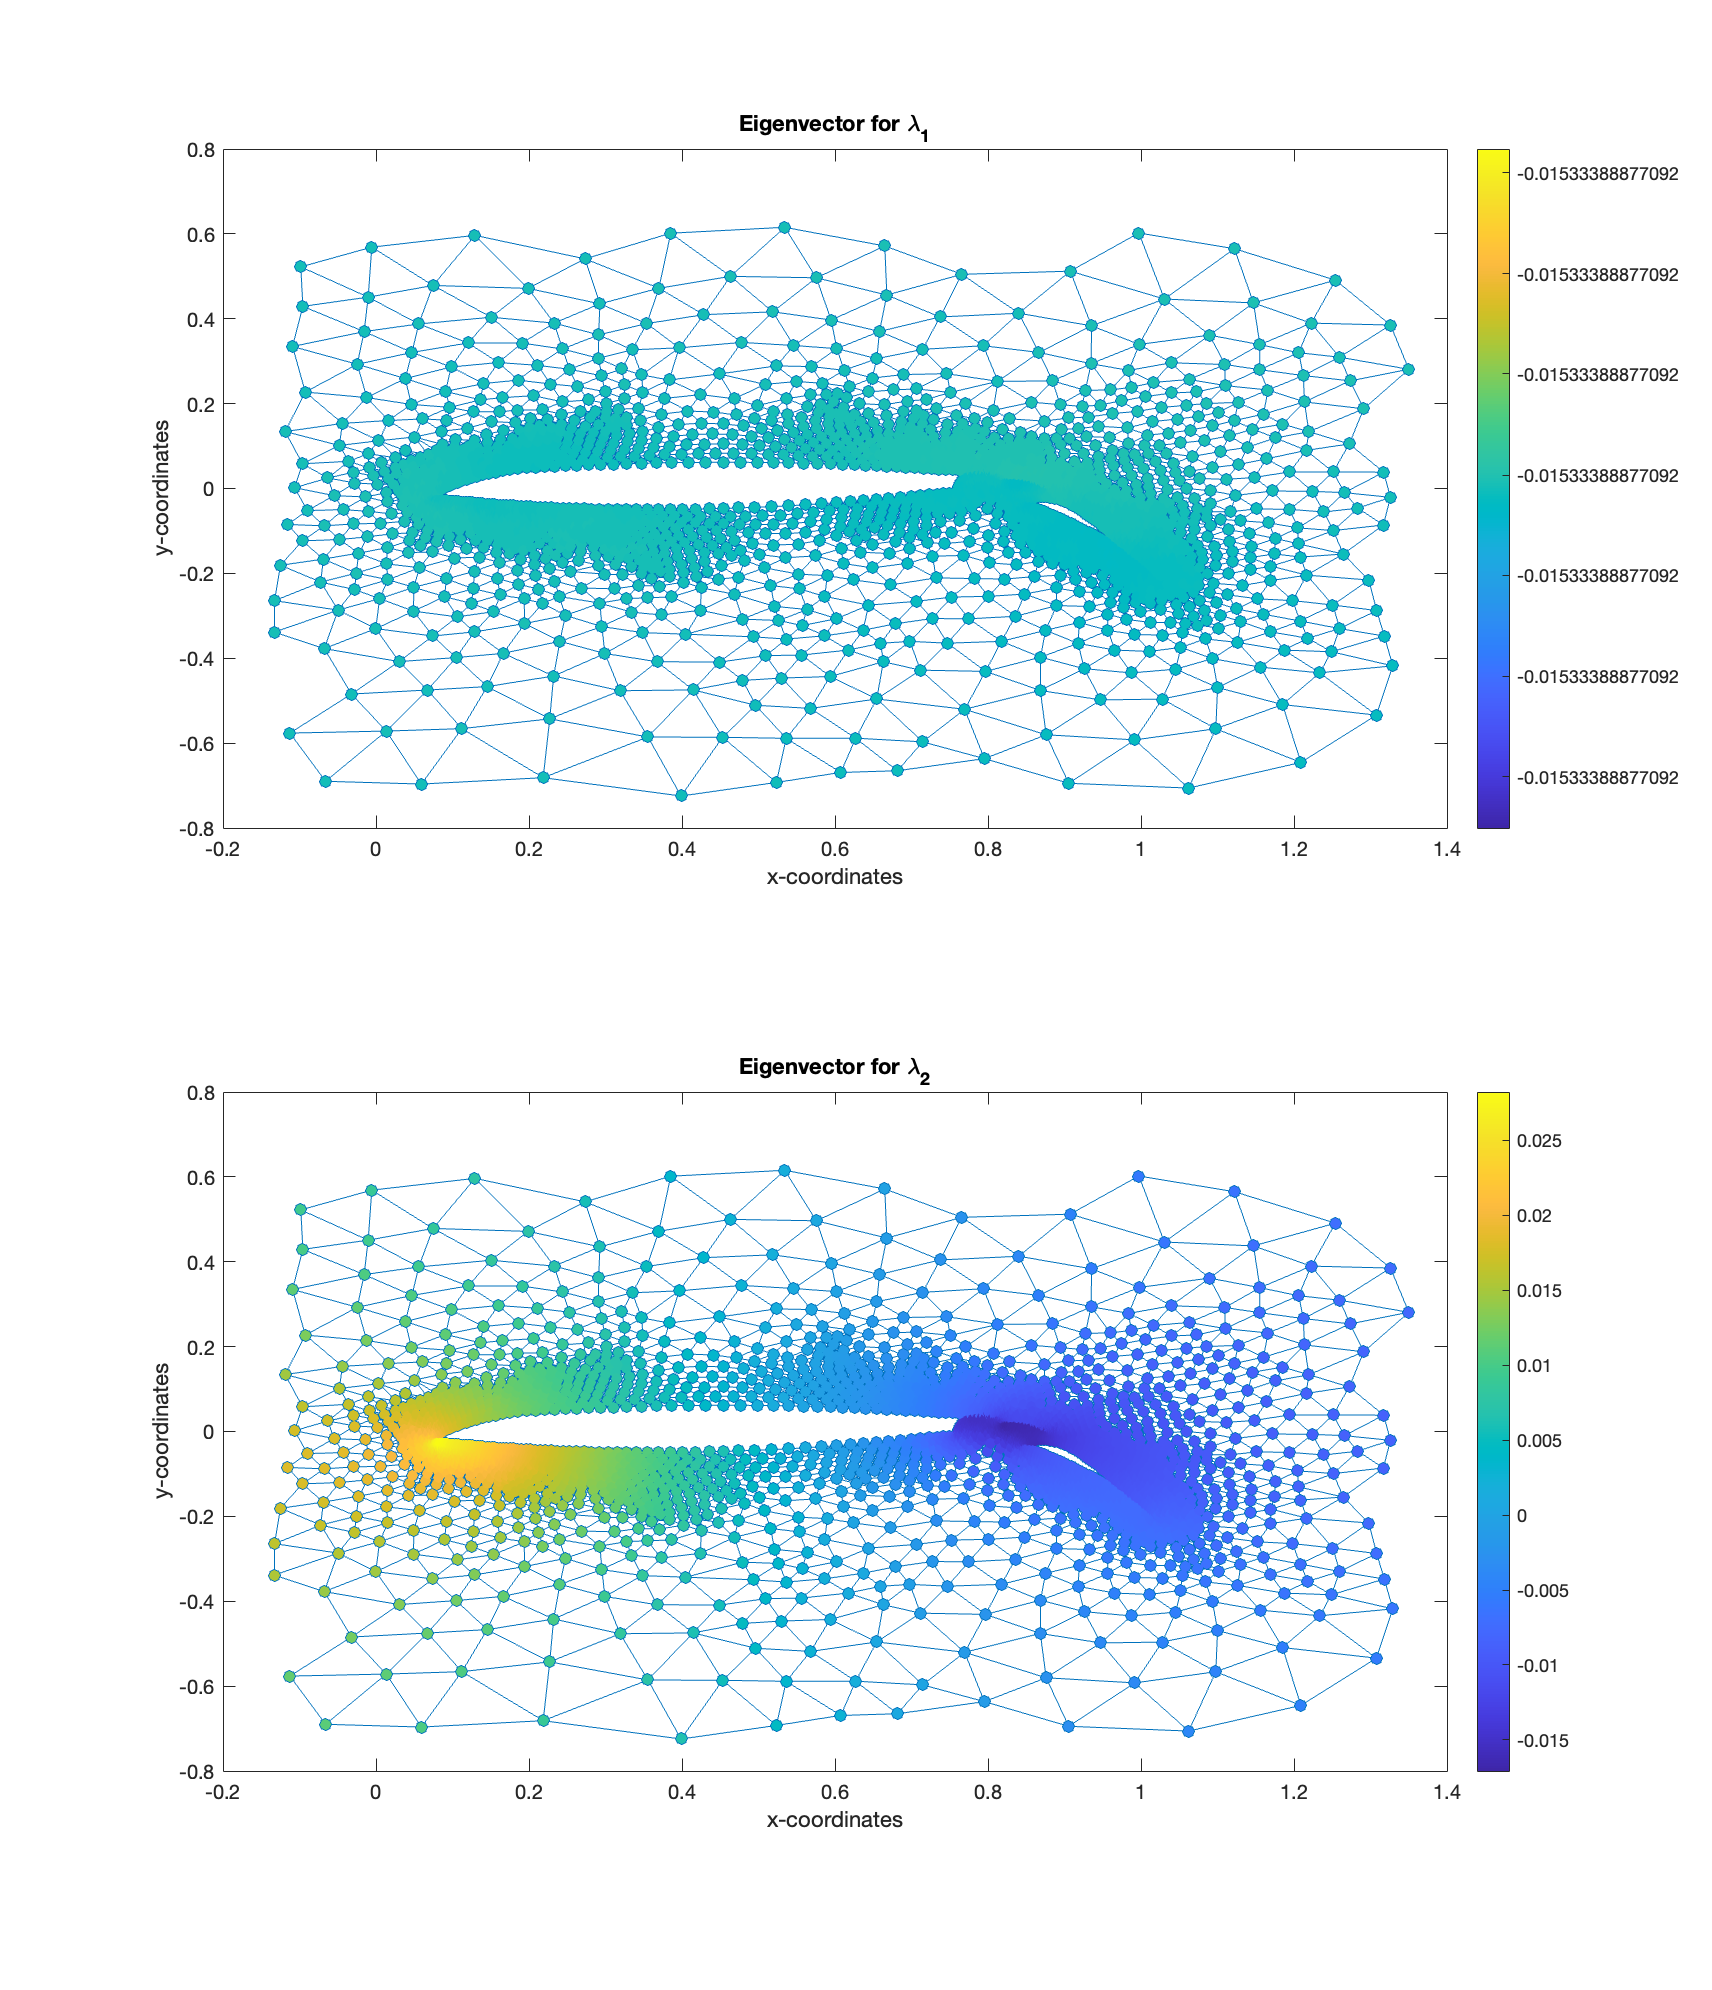
\includegraphics[width=\textwidth]{./media/eigenvector.png}
		\caption{The vertices colored according to their corresponding eigenvector element}
		\label{sfig:eig1}
	\end{subfigure}%
	~
	\begin{subfigure}{0.5\textwidth}
		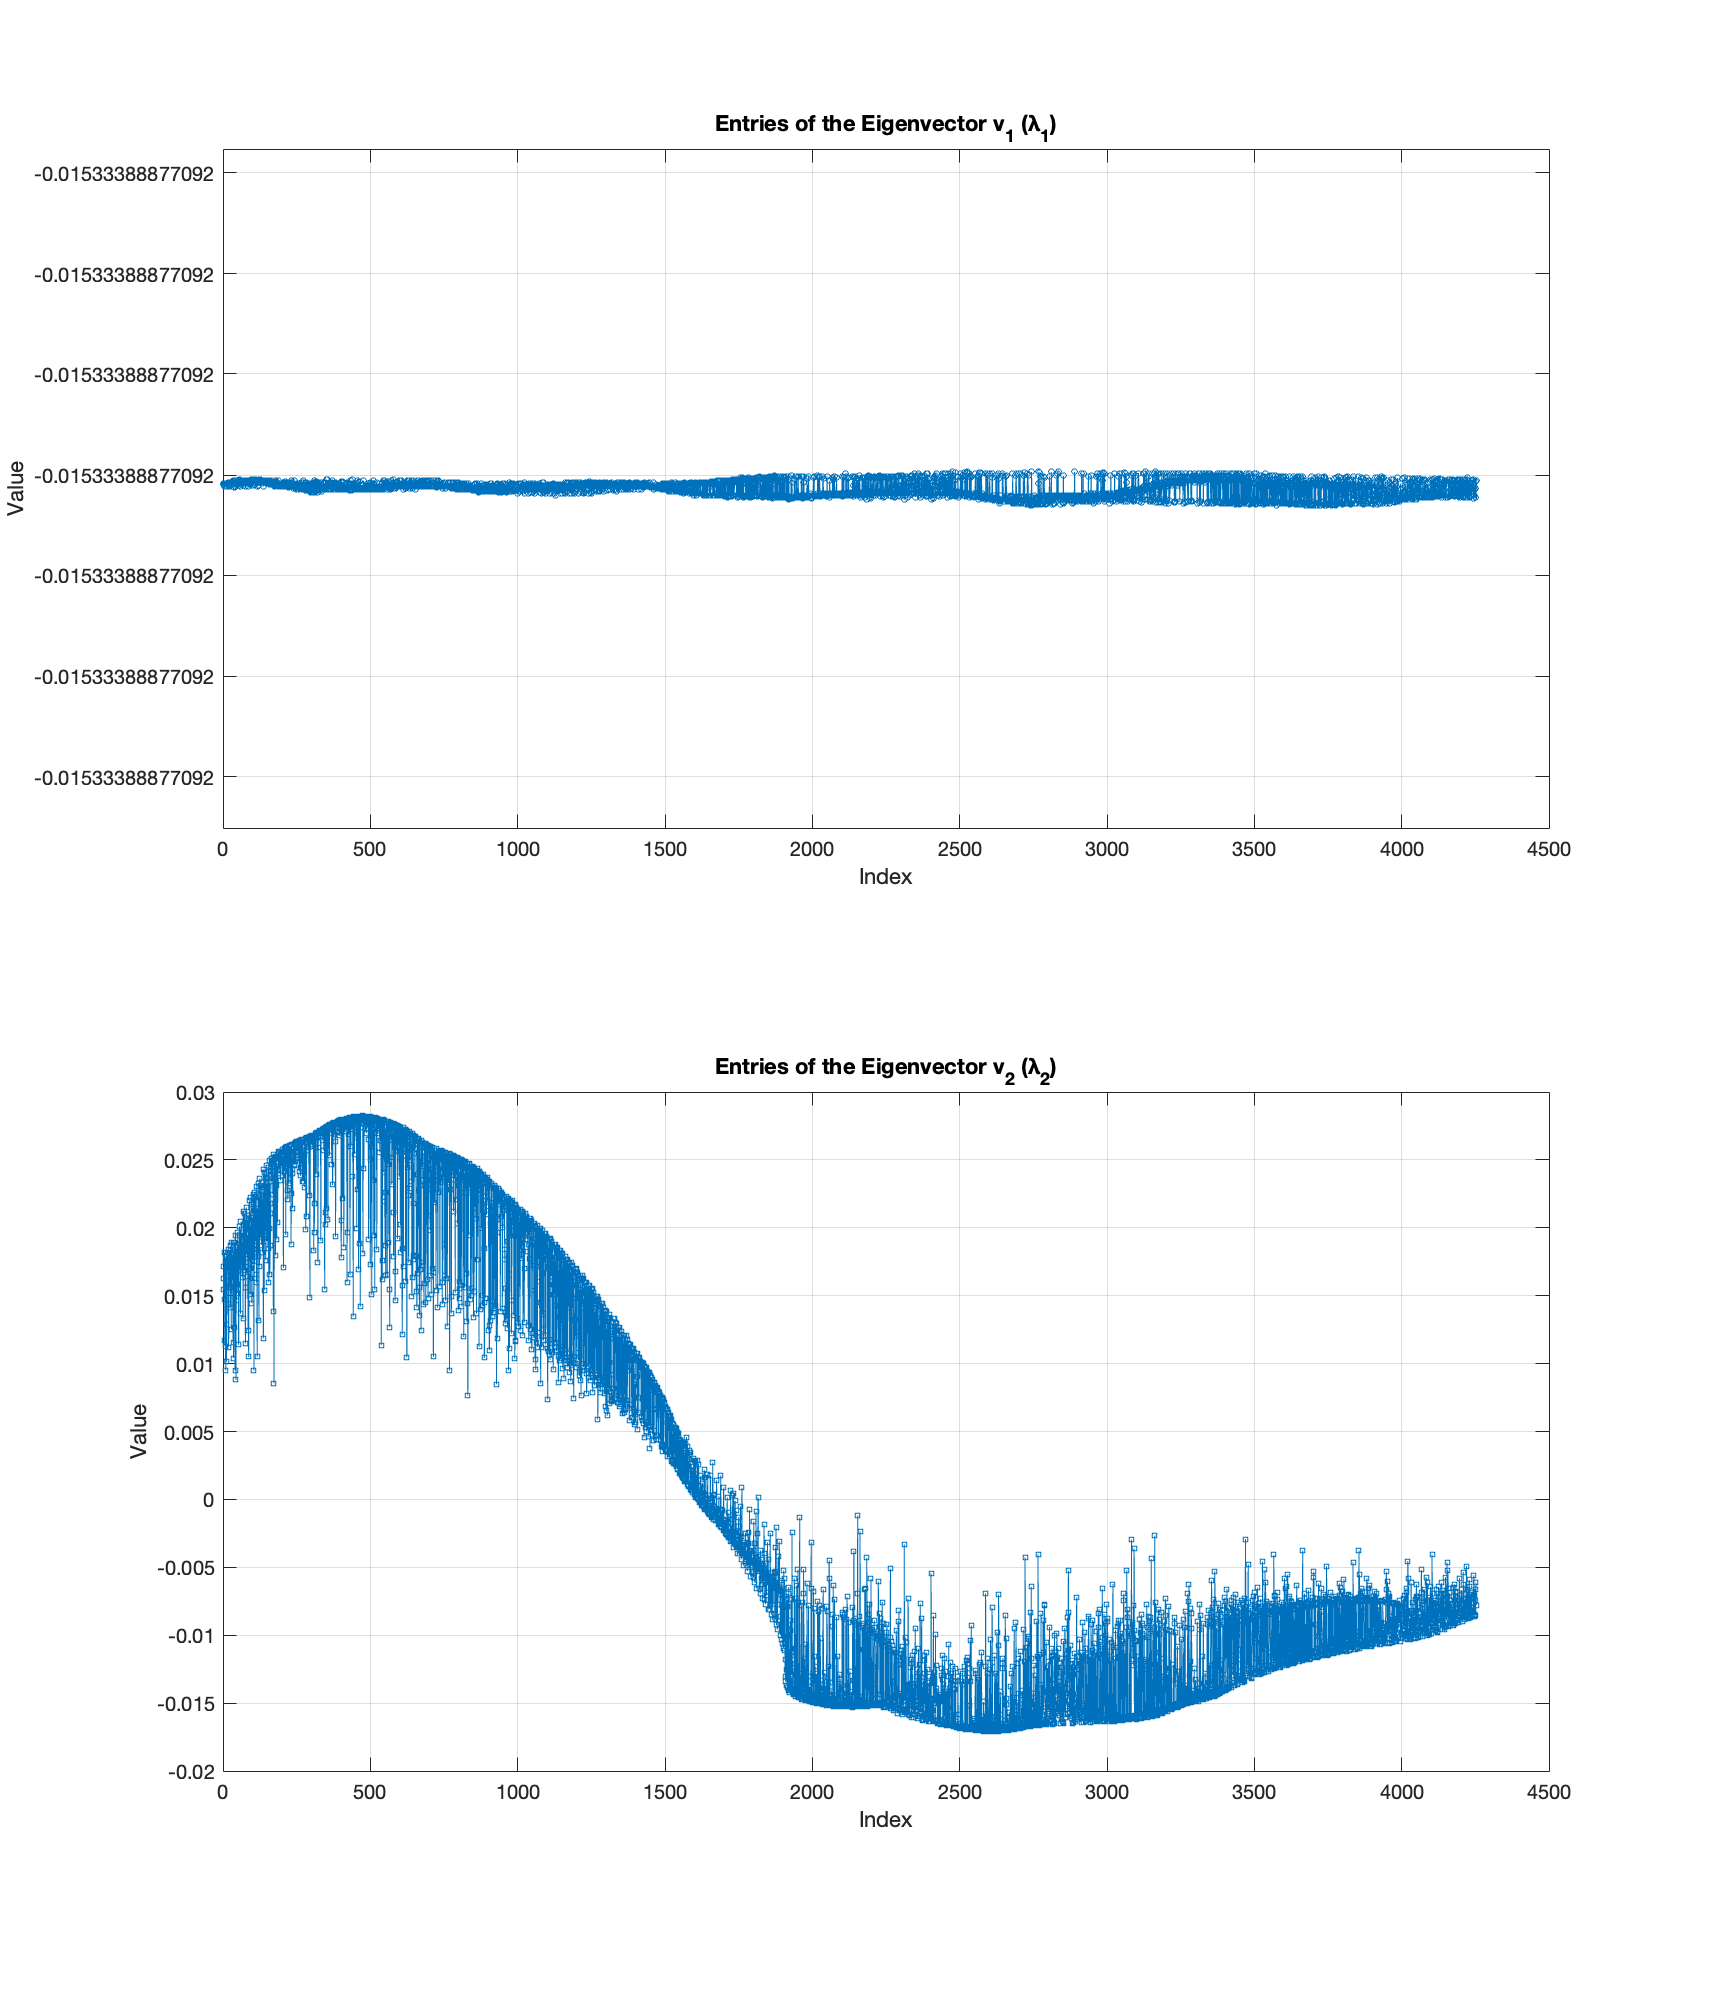
\includegraphics[width=\textwidth]{./media/eig_2.png}
		\caption{The entries of the eigenvector plotted against their indices. }
		\label{sfig:eig2}
	\end{subfigure}\\
	\caption{Entries of the eigenvector associated with the first ($\lambda_1$)} and second ($\lambda_2$) smallest eigenvector.
	\label{fig:eig}
\end{figure}
As the next step we project each solution on the coordinate system space for the graph mesh3e1, barth4, 3elt and crack The result of this can be seen in Figure~\ref{fig:proj}. Looking at the shape of the values of the fiedler vector we can see that the for 3elt and barth4, they are concentrated in a vertical transition.
While for the other two, they have more of a planar structure, creating a clear horizontal separation. Furthermore all graphs appear to have a smooth transition, seen by the transition of color from dark blue to red.
\newline
\newline
As the final step show the graph with its partitions and edge cut by not using the coordinate space, but by using the eigenvectors values of the graph Laplacian.
In Figure~\ref{fig:eig_spc} one can see the partitioning results in two ways. On the top using the eigenvector values and on the bottom the Euclidean coordinates. For the barth4 mesh for example in Subfigure \ref{fig:barth4_spc} we are able to visualize the relation between nodes a lot more effectively using the eigenvector values as our coordinates, in comparison to the cartesian version, where the groups are barely visible. 
\begin{figure}[H]
	\centering
	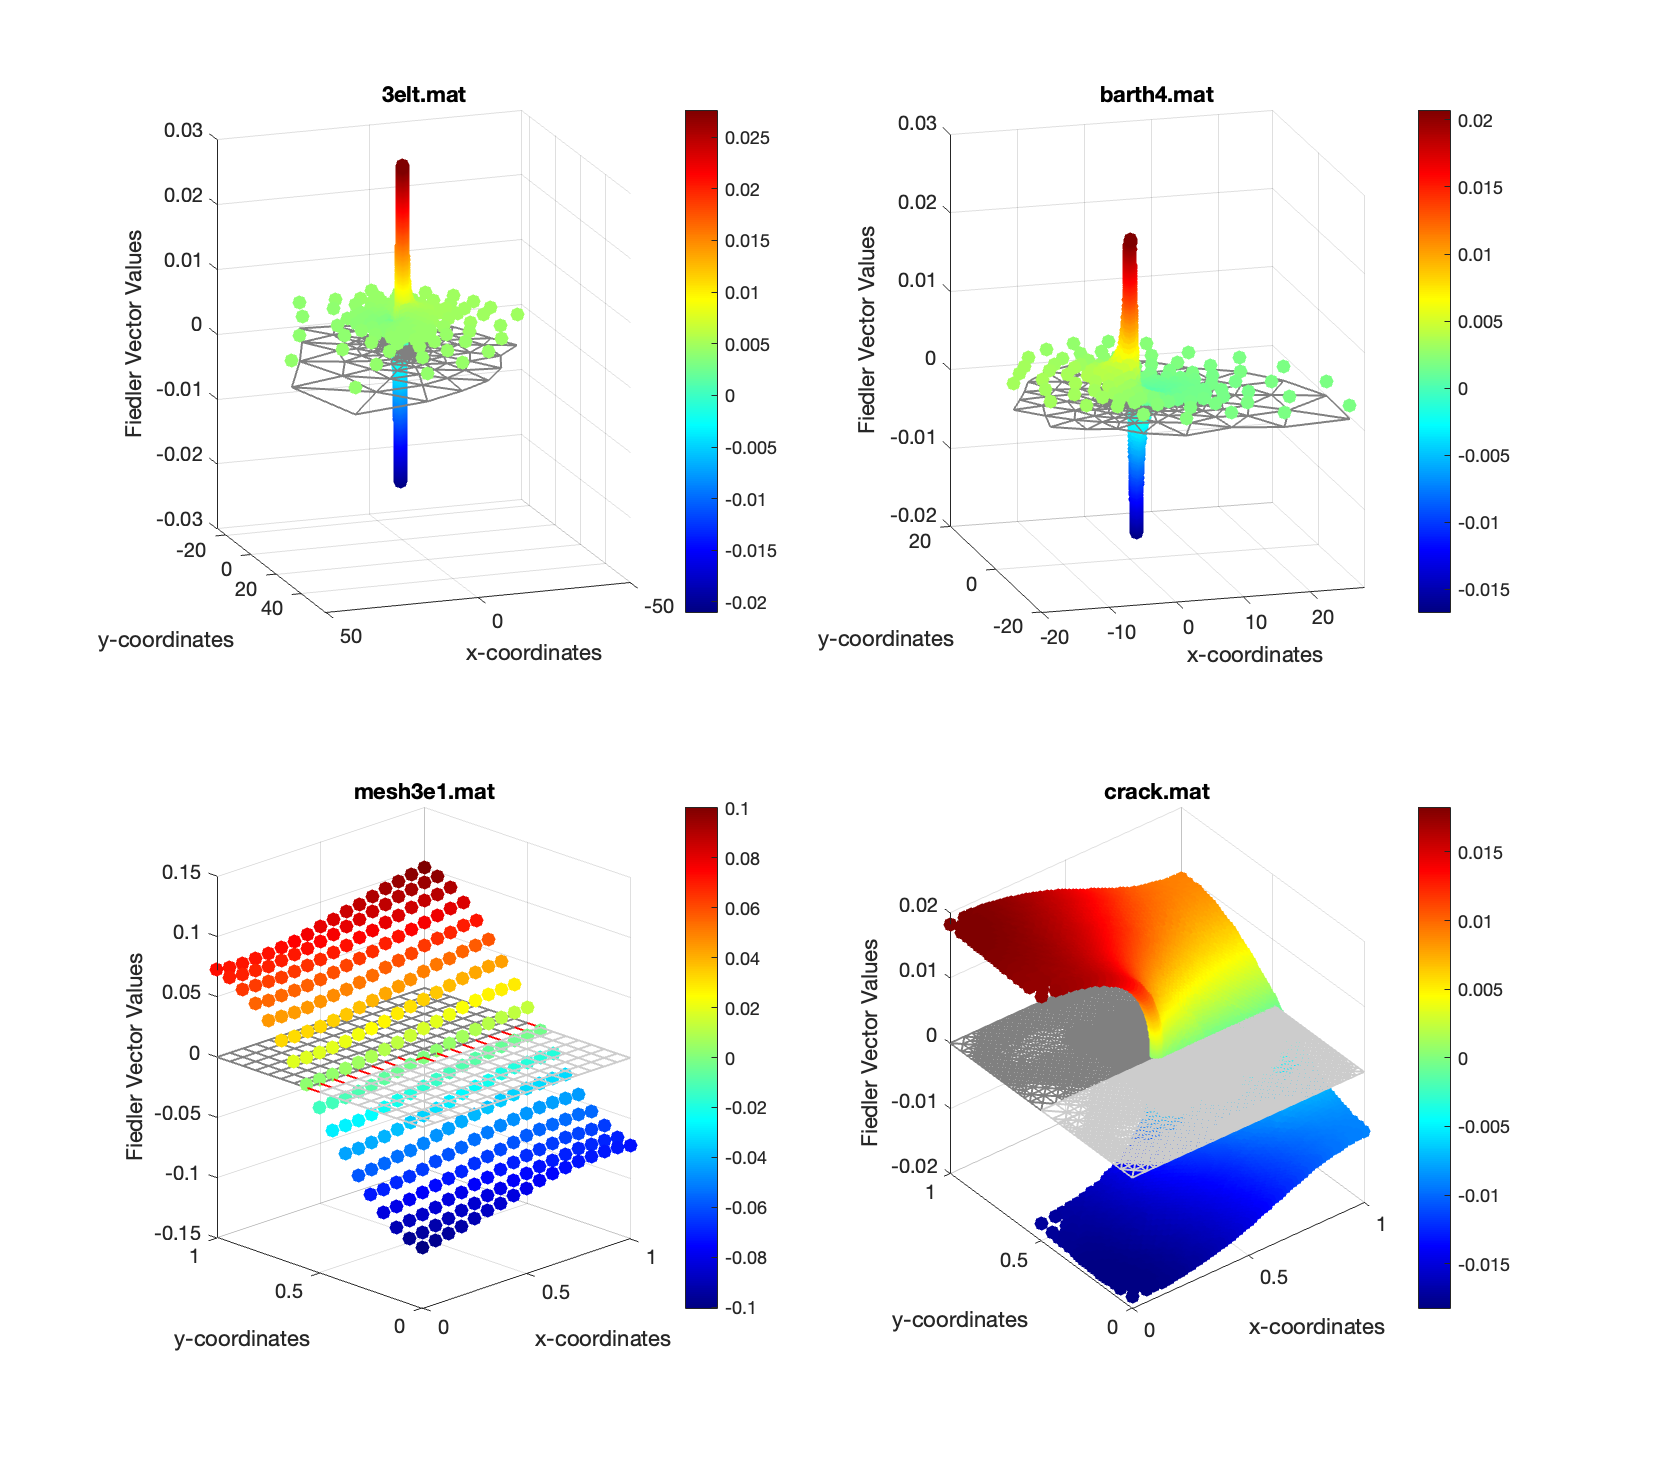
\includegraphics[width=\textwidth]{./media/fiedler.png}
	\caption{Entries of the eigenvector associated with the second smallest eigenvalue $\lambda_2$ of the Graph Laplacian matrix $L$. The two partitions are depicted in dark gray and light gray, while the cut edges is red respectively. The z-axis represents the value of the entries of the eigenvector. }
	\label{fig:proj}
\end{figure}

\begin{figure}[H]
	\centering
	\begin{subfigure}{0.5\textwidth}
		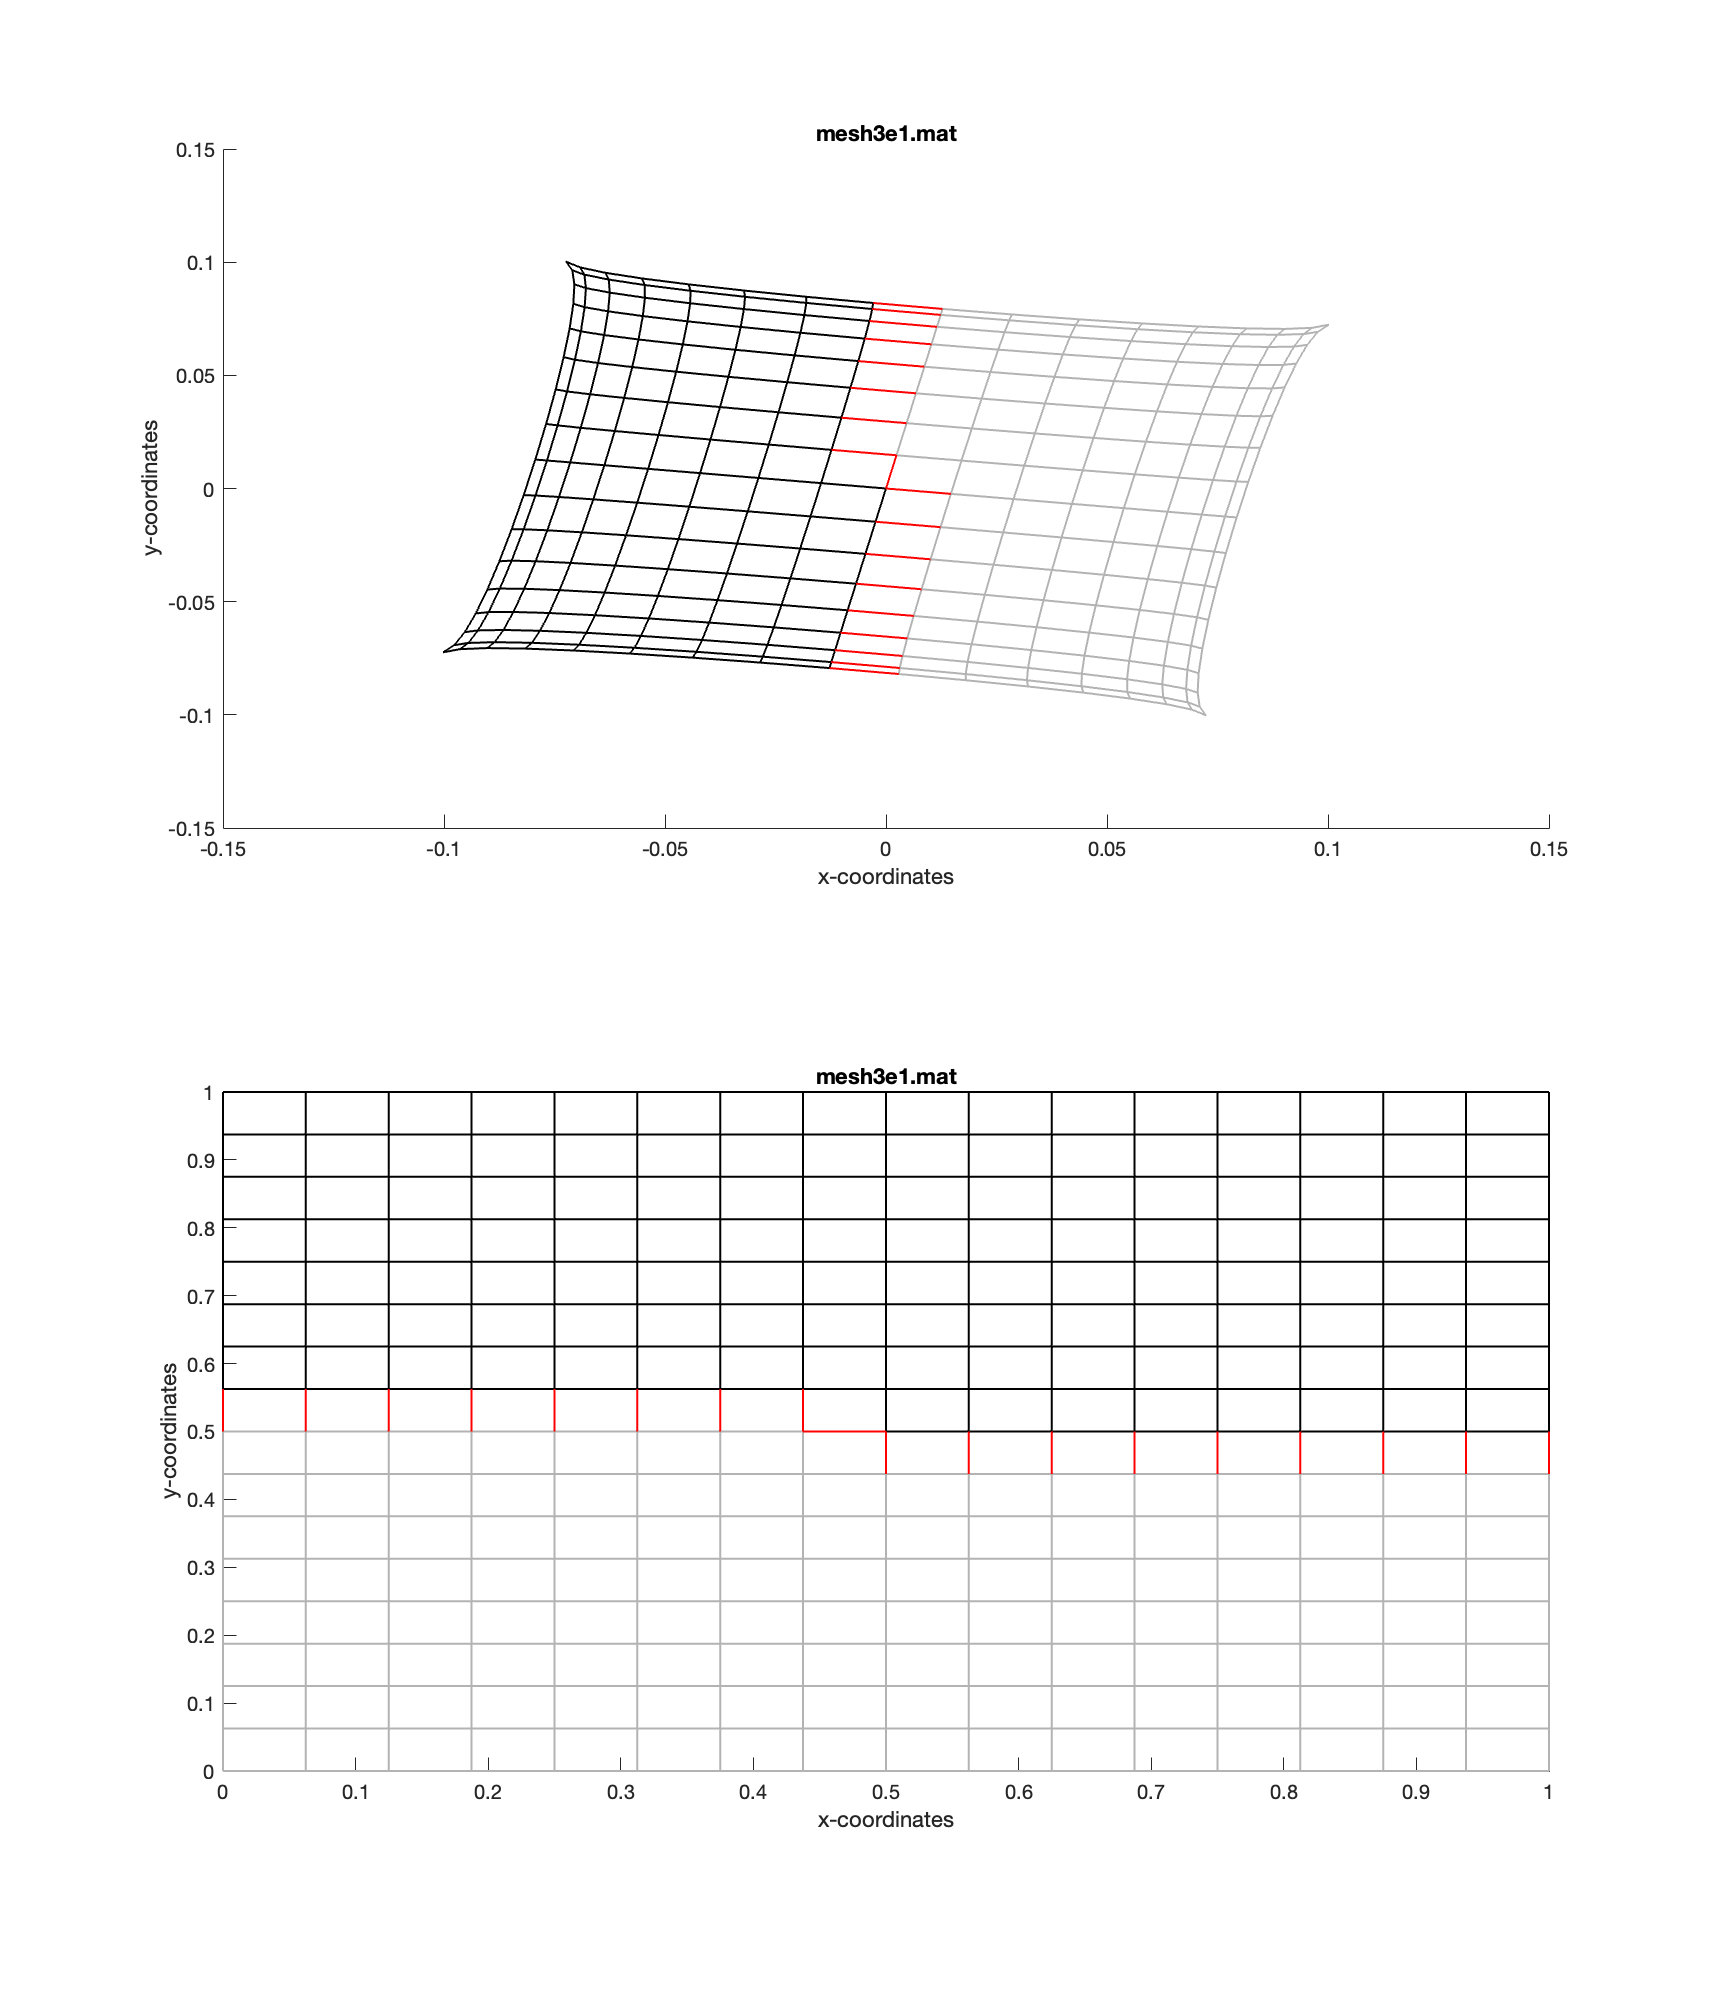
\includegraphics[width=\textwidth]{./media/mesh3e1_eigen.png}
		\caption{mesh3e1}
		\label{fig:spec_crack}
	\end{subfigure}%
	~
	\begin{subfigure}{0.5\textwidth}
		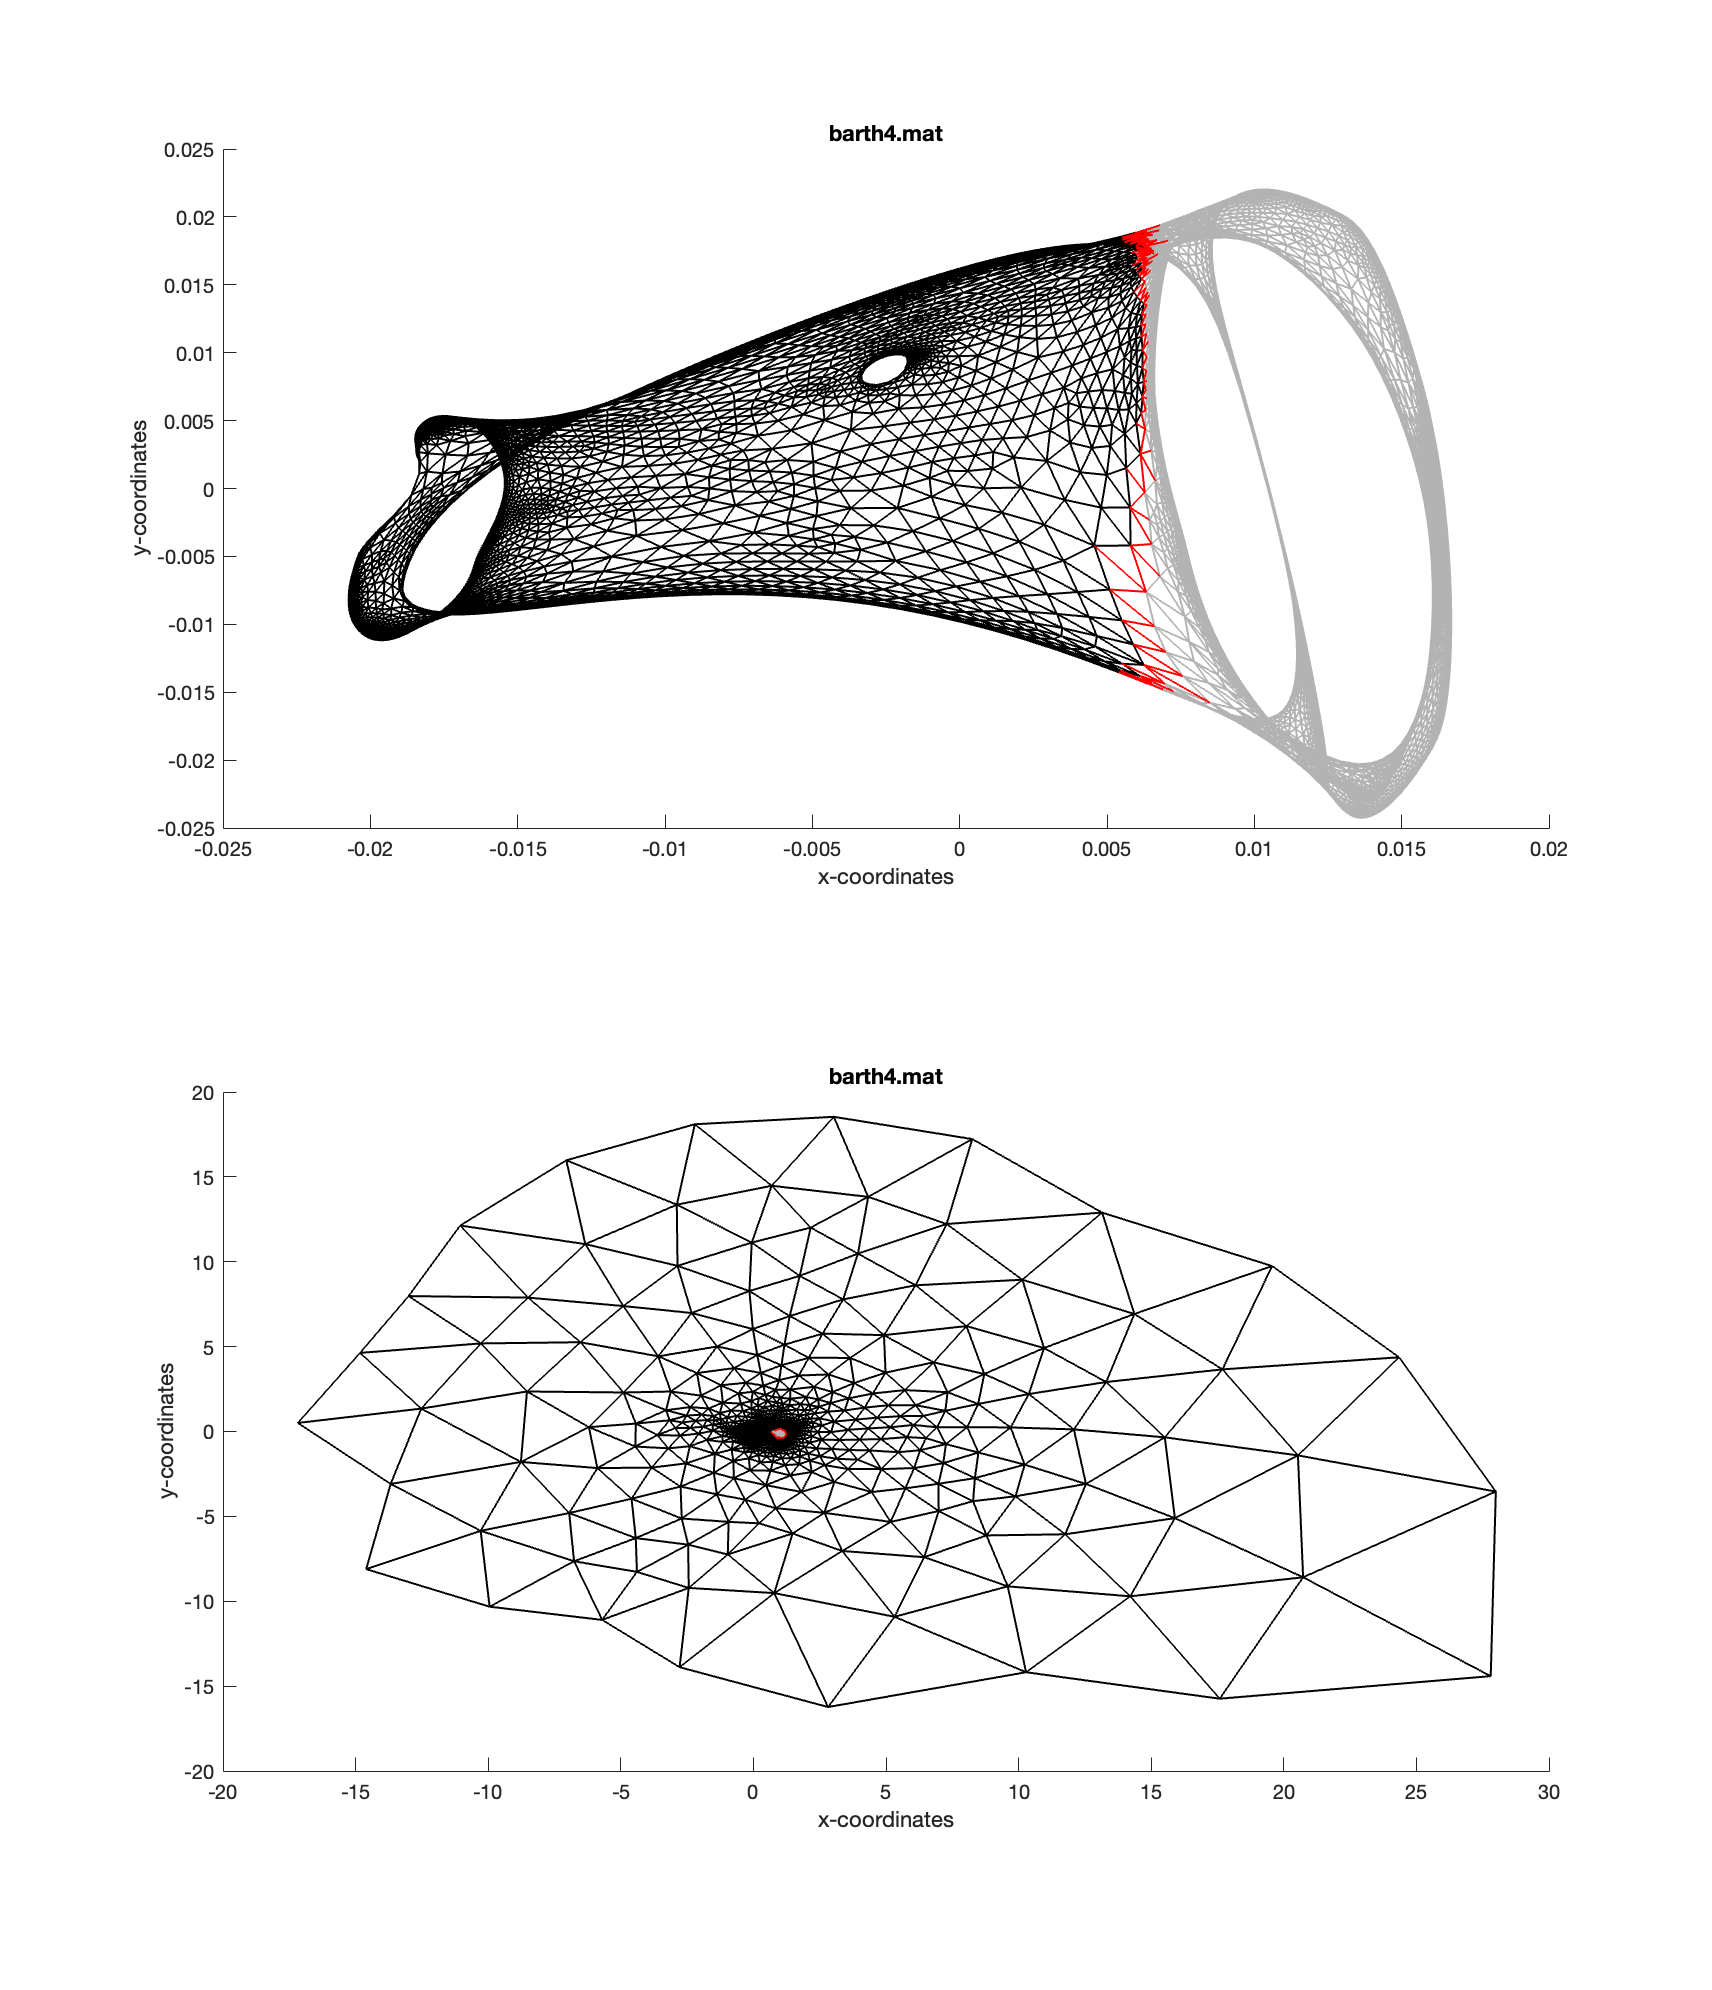
\includegraphics[width=\textwidth]{./media/barth4_eigen.png}
		\caption{barth4}
		\label{fig:barth4_spc}
	\end{subfigure}\\
	\begin{subfigure}{0.5\textwidth}
		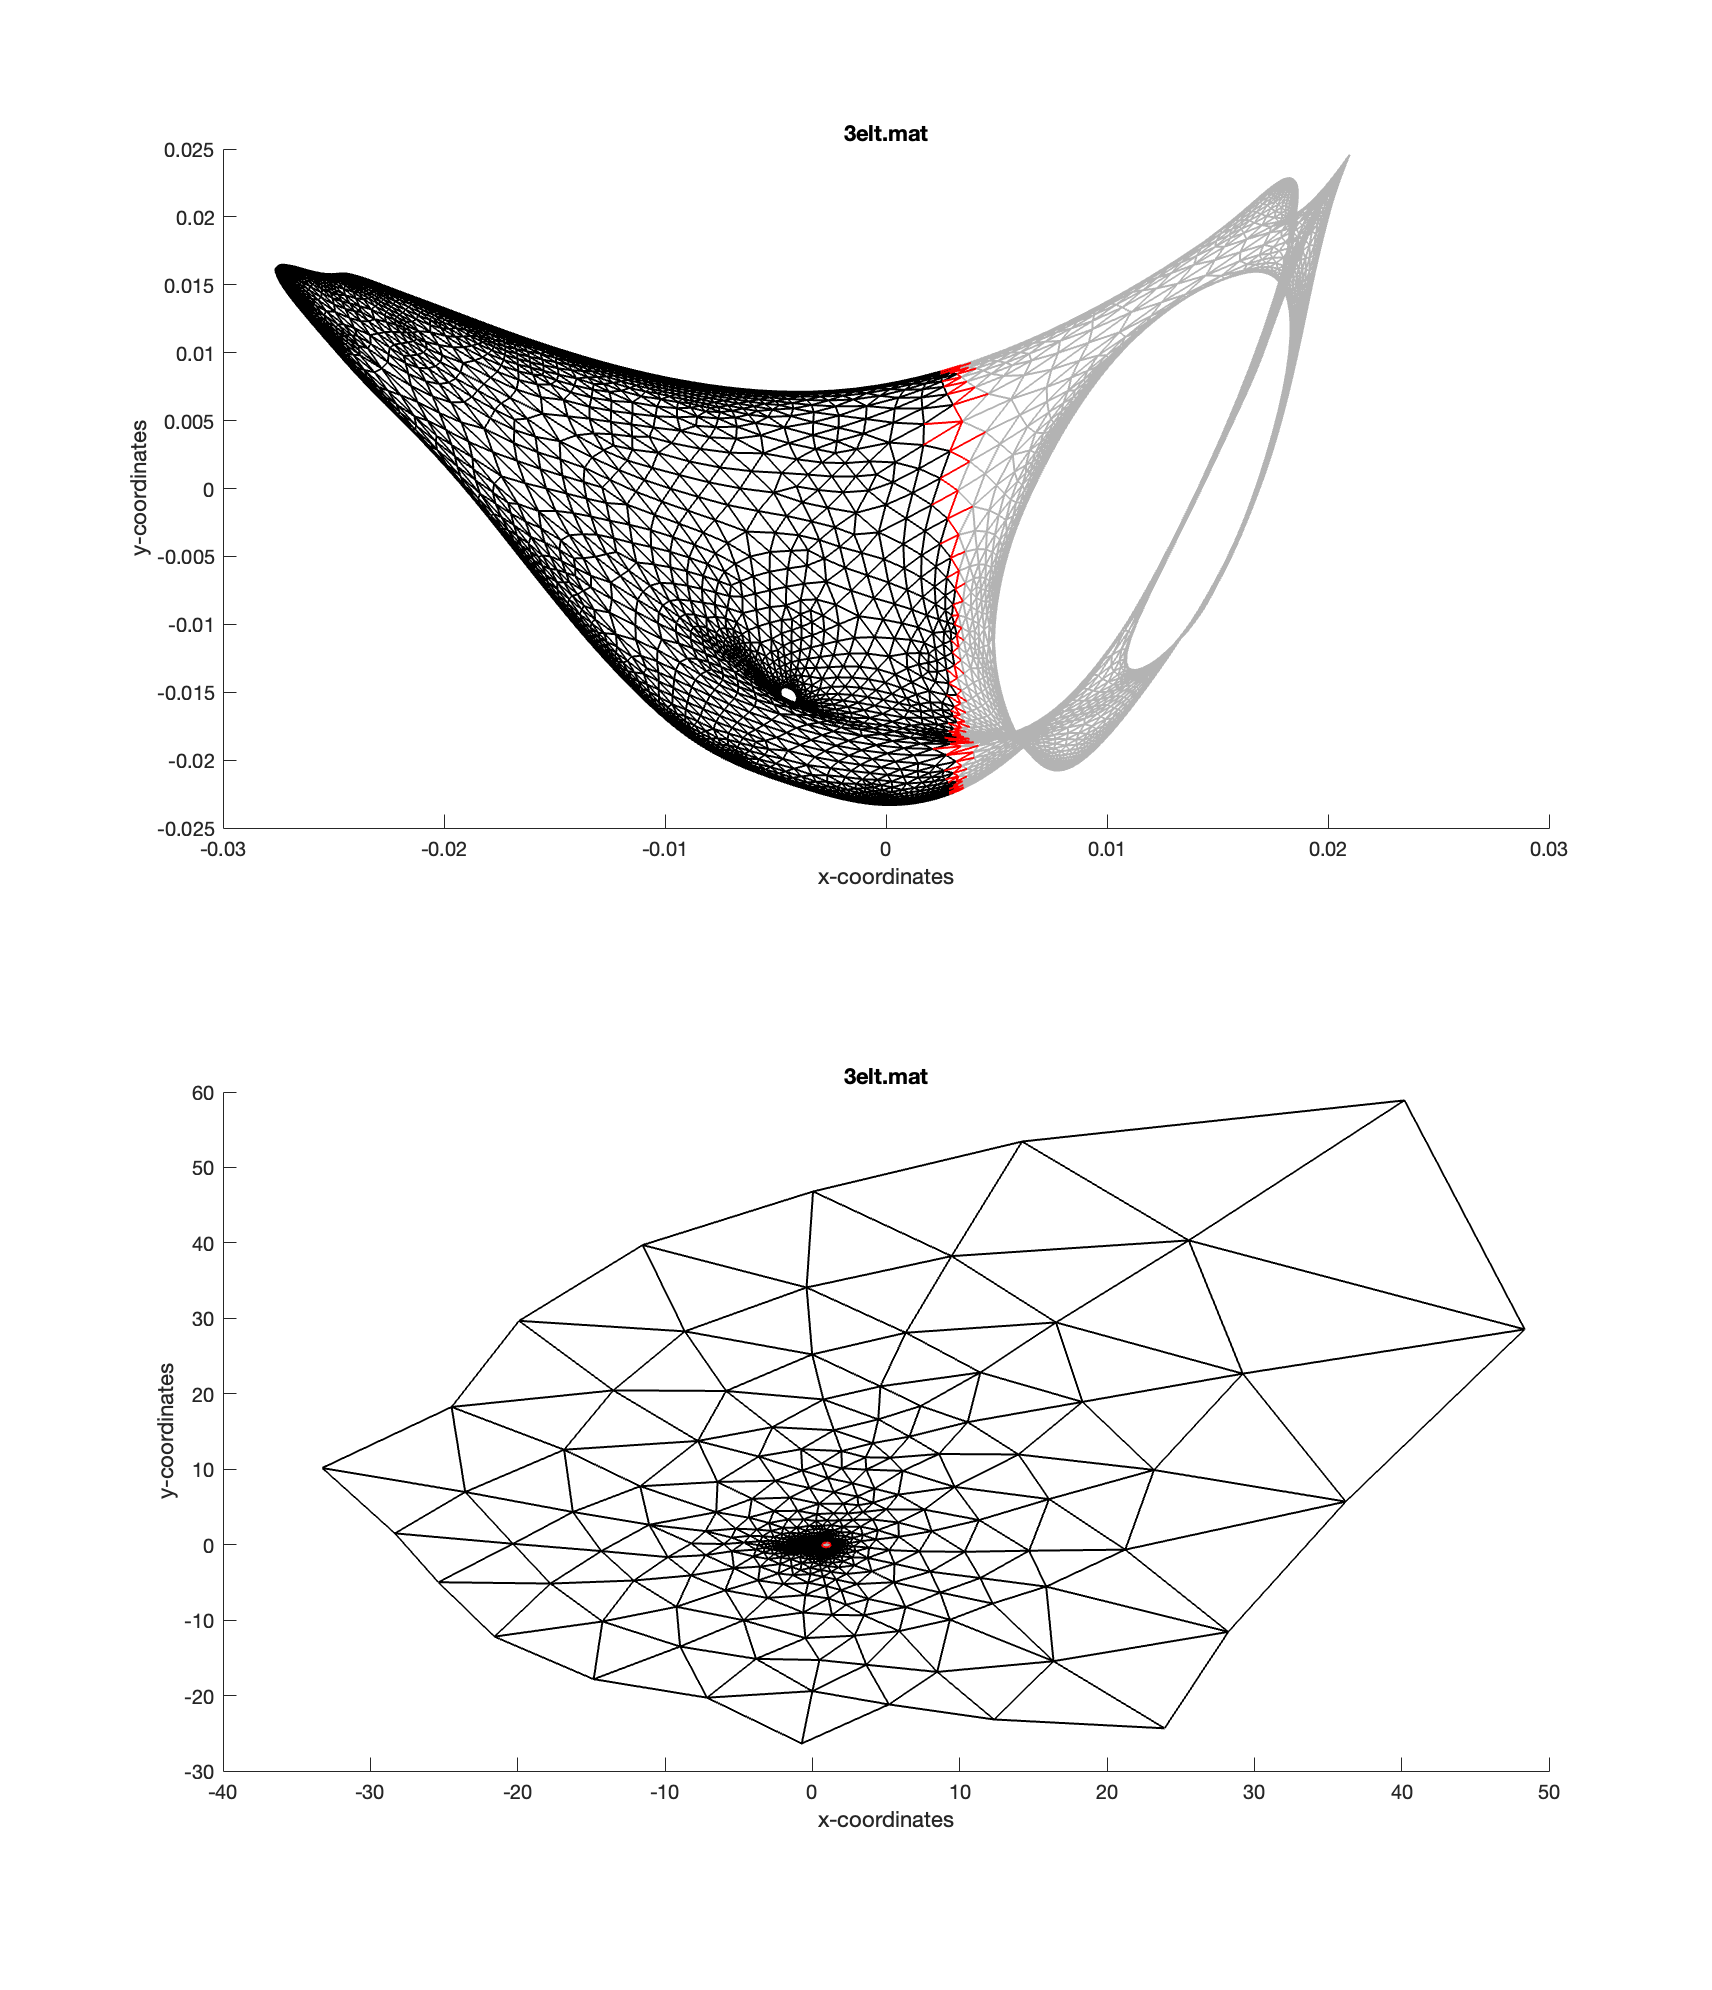
\includegraphics[width=\textwidth]{./media/3elt_eigen.png}
		\caption{3elt}
		\label{fig:metis_crack}
	\end{subfigure}%
	~
	\begin{subfigure}{0.5\textwidth}
		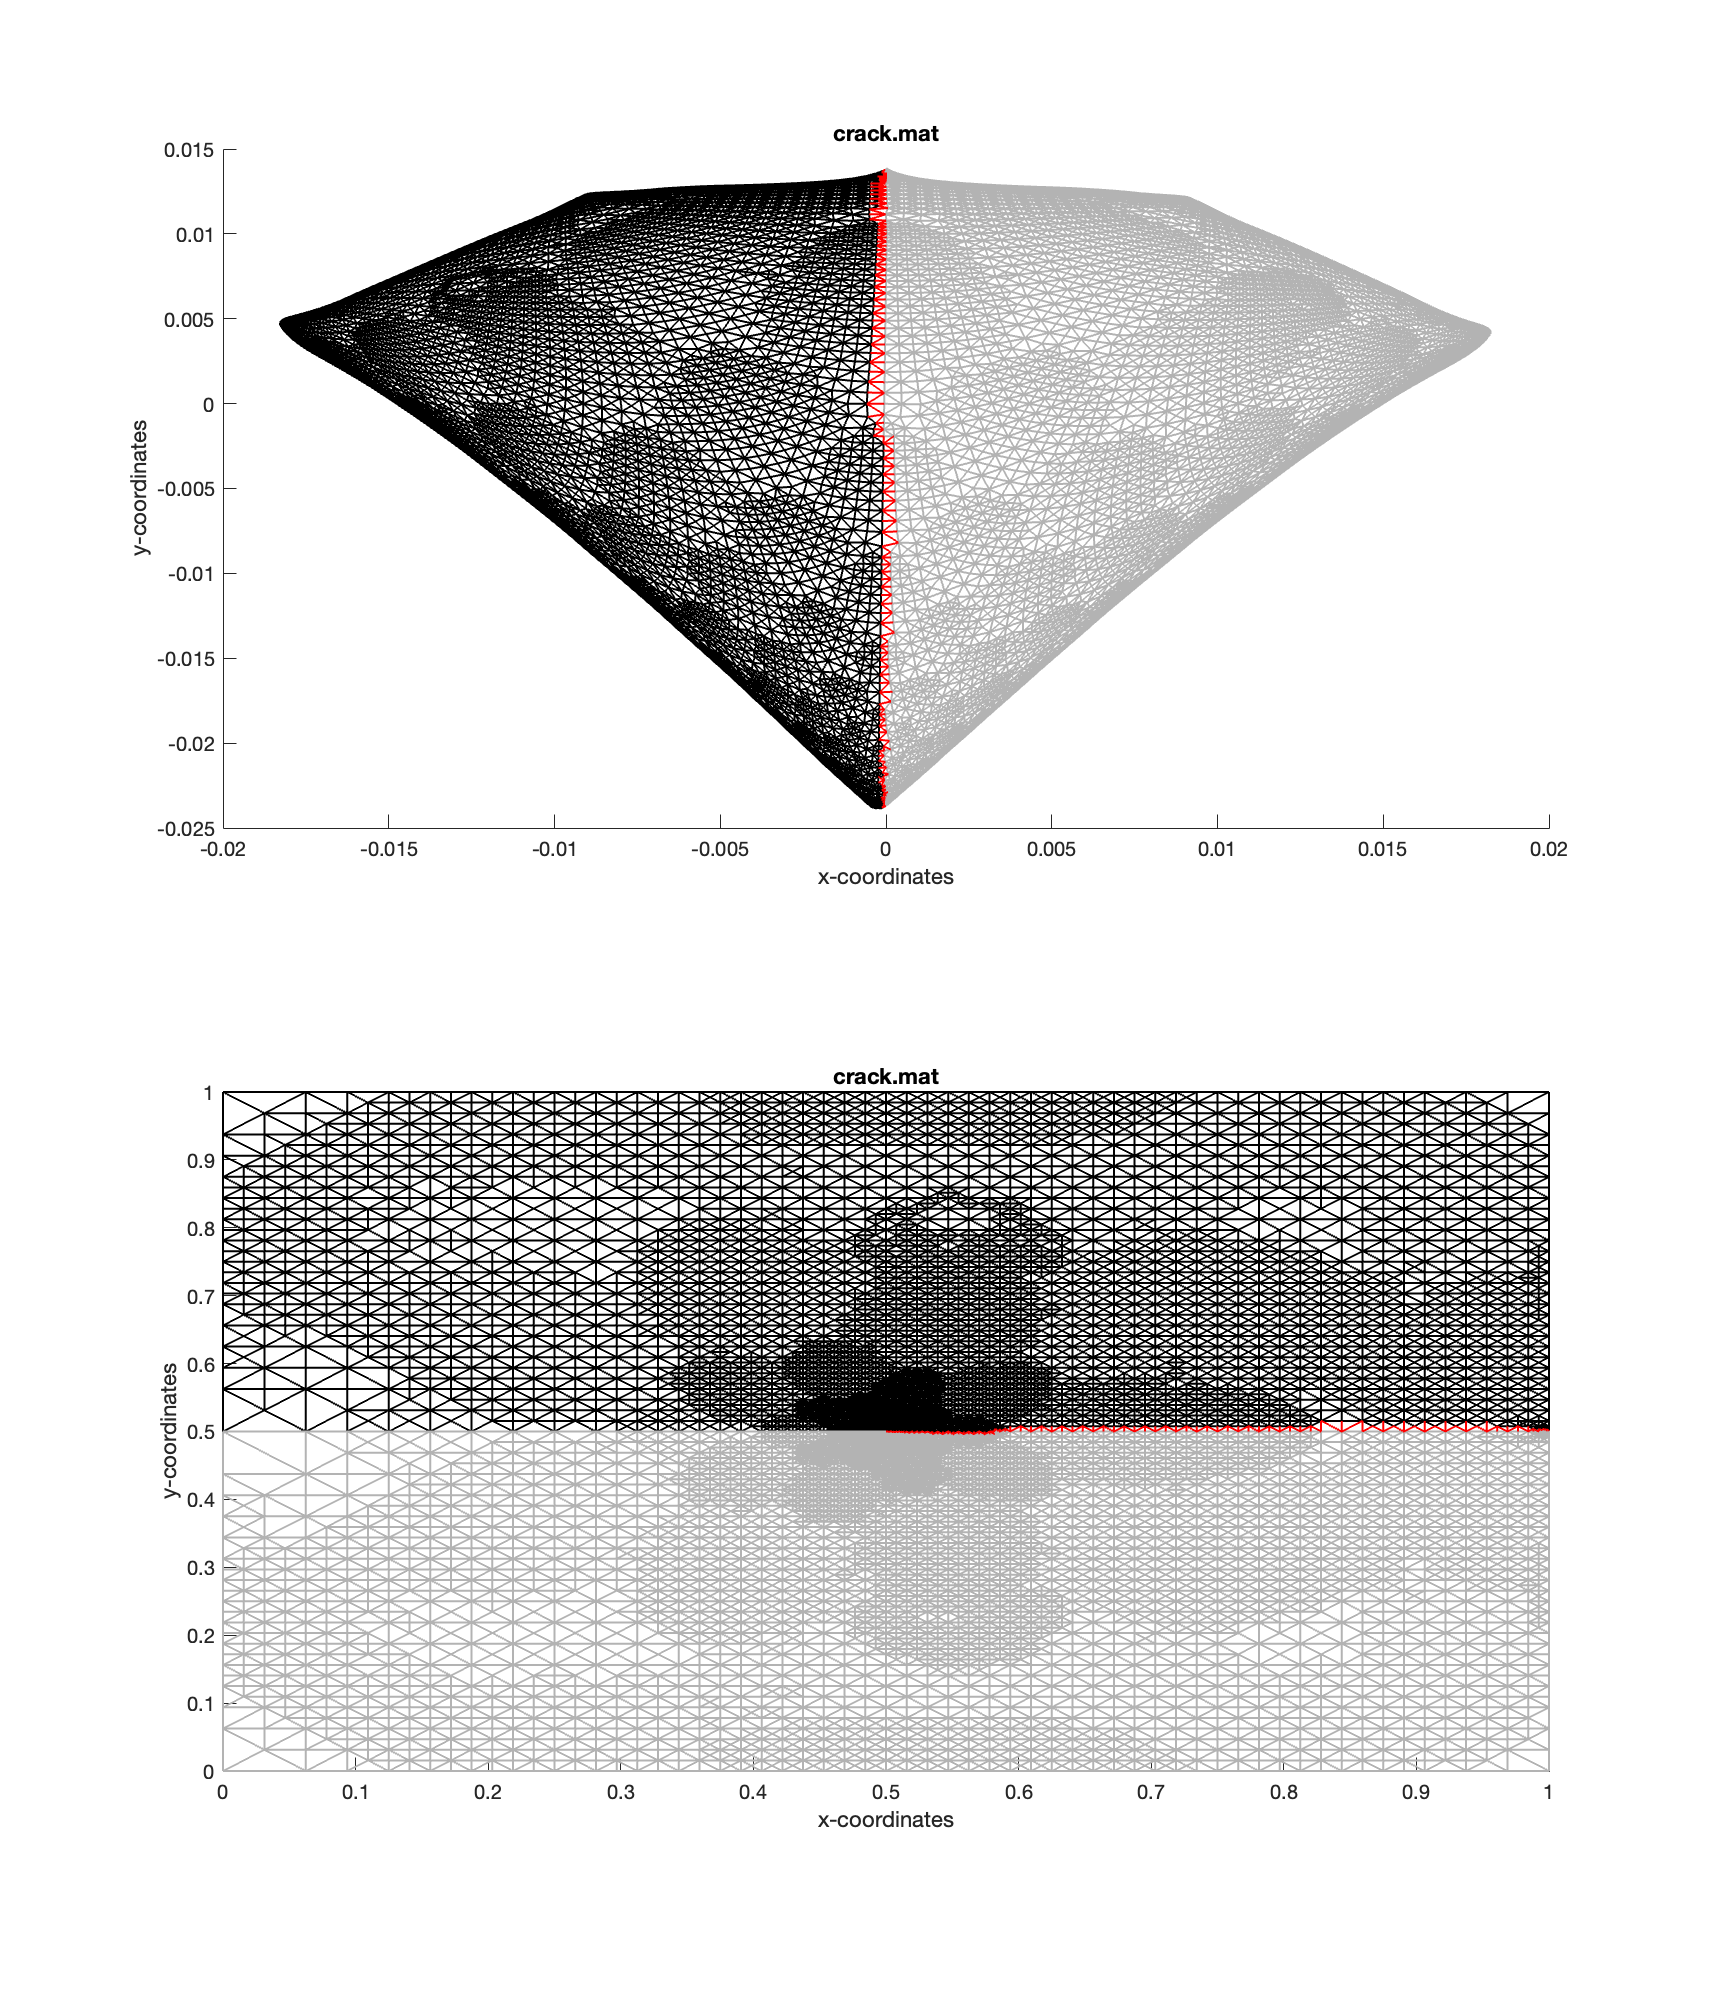
\includegraphics[width=\textwidth]{./media/crack_eigen.png}
		\caption{crack}
		\label{fig:inert_crack}
	\end{subfigure}
	\caption{Spectral bi-partitioning results using the eigenvectors to supply coordinates (top) and using cartesian coordinates (bottom).}
	\label{fig:eig_spc}
\end{figure}



% \newpage
\printbibliography[heading=bibintoc]
\end{document}
